\chapter{Эксперименты} \label{chapt3}

Описанные в главах \ref{chapt1} и \ref{chapt2} алгоритмы имеют значительное
количество параметров. Для подбора их оптимальной комбинации, фактически,
необходимо решить задачу многомерной оптимизации в достаточно большом
пространстве. Очевидно, что в данном случае невозможно решить эту задачу
аналитически. Также невозможно перебрать все возможные комбинации параметров
ввиду слишком большого их числа. Однако во многих случаях можно определить
разумный диапазон возможных значений параметра и исследовать изменение качества
распознавания аккордов в зависимости от значений данного параметра в указанном
диапазоне.

Применение методов вычисления классификации векторов признаков, основывающихся
на машинном обучении, не позволяет целиком избавиться от ручного подбора
параметров. Во-первых, эти алгоритмы могут иметь метапараметры, не изменяемые в
процессе обучения (например, количество нейронов в $j$-м слое нейронной сети).
Во-вторых, параметры имеются также на этапах подготовки входных данных и
интерпретации результата.

Поскольку все эксперименты проводились на описанной в разделе \ref{ssect3_coll}
коллекции из 318 музыкальных звукозаписей, найденные значения параметров будут
оптимальными только для этой коллекции. Способствовать преодолению этой проблемы
могли бы достаточно большие коллекции аннотированных композиций, не существующие
на данный момент.

Все эксперименты можно разделить на 4 группы. В разделе \ref{sect3_spectcalc}
рассматривается этап предварительной обработки звукозаписи и получения
спектрограммы. В разделе \ref{sect3_specttrans} исследуется влияние различных
преобразований спектрограммы на качество распознавания аккордов. Эксперименты
в разделе \ref{sect3_nn} направлены на отыскание наилучших параметров нейронной
сети, используемой для получения признаков. Преобразования над
последовательностями векторов признаков и распознанных аккордов и параметры
выбранного метода классификации анализируются в разделе \ref{sect3_class}. В
разделе \ref{sect3_time} сравниваются скорости работы реализованных алгоритмов.

В экспериментах были использованы следующие значения параметров (если явно не
указано иное):
\begin{itemize}
  \item $N_0 = 36$;
  \item частотный диапазон от 65,4 Гц (нота \emph{до} большой октавы) до 987,77
  Гц (нота \emph{си} второй октавы);
  \item $T = 8$;
  \item $w = 15$;
  \item $d = 100$ мс;
  \item $\eta = 50000$;
  \item $\xi = 15$;
  \item $\zeta = 0.1$;
  \item количество учитываемых гармоник -- 3;
  \item $h = 0.6$;
  \item $L_N = 0.002$.
\end{itemize}

\section{Оценка качества распознавания аккордов} \label{sect3_eval}

Поскольку алгоритмы распознавания аккордов предназначаются для обработки
музыкальных звукозаписей, необходимо оценивать качество их работы на реальных
звукозаписях, а не на искусственно сгенерированных примерах. Чтобы звукозапись
можно было использовать для оценки, требуется вручную решить задачу
распознавания последовательности аккордов, то есть для каждого момента времени
$t \in [t_{start}, t_{end}]$ указать аккорд $y \in \overline{Y}$, звучащий в
этот момент. При этом набор $\overline{Y}$ включает в себя все возможные в
музыке сочетания нот и отдельные ноты. Также требуется с высокой точностью
указать моменты начала и конца звучания аккордов. Всё это делает задачу
подготовки тестовых коллекций очень трудоёмкой.

Для хранения этой информации используют особым образом отформатированные
текстовые файлы, называемые файлами разметки или файлами текстовых аннотаций.
Ниже приведён пример такого файла:
\begin{lstlisting}
0.000	0.848	N
0.848	1.625	A:min
1.625	3.017	G:maj
3.017	3.895	F:maj
...
\end{lstlisting}
Первый и второй столбцы содержат время начала и конца звучания аккорда
соответственно, в третьем столбце записывается название аккорда. 

\subsection{Коллекции текстовых аннотаций} \label{ssect3_coll}

На текущий момент существует 5 коллекций текстовых аннотаций для популярной
музыки разных исполнителей:
\begin{itemize}
  \item \emph{Isophonics} \cite{MauchOmp2009}. Текстовые аннотации для 180
  композиций (12 альбомов) \textit{The Beatles}, 20 композиций \textit{Queen}
  (с альбома \textit{Greatest Hits}), 18 композиций \textit{Zweieck} (с альбома
  \textit{Zweilicht}). Наиболее часто используется для исследований, несколько
  раз использовалась для ежегодных соревнований MIREX Audio Chord Estimation.
  
  \item \emph{RWC Pop Music} \cite{Goto2002}. Текстовые аннотации для 100
  композиций японской и западной популярной музыки.
  
  \item \emph{Billboard} \cite{Burgoyne2011}. Текстовые аннотации для 197
  композиций из американского чарта \textit{Billboard 100} за промежуток с 1958
  по 1991 год. Использовалась в соревновании MIREX Audio Chord Estimation в 2012
  году.
  
  \item \emph{uspop2002} \cite{Berenzweig2004}. Текстовые аннотации для 195
  композиций американской популярной музыки.
  
  \item \emph{Robbie Williams annotations}. Текстовые аннтоации для 65
  композиций \textit{Robbie Williams} (первые 5 альбомов).
\end{itemize}

Поскольку в аннотациях указывается точное время, важно при анализе использовать
точно те же версии звукозаписей, которые были использованы при подготовке
аннотаций. Это затрудняет использование некоторых коллекций. Для тестирования
алгоритмов в рамках данной работы использовались коллекции \emph{Isophonics} и
\emph{RWC Pop Music}.

\subsection{Сопоставление последовательностей аккордов}

Вопросом оценки того, насколько одна последовательность аккордов (определённая
автоматически) соответствует другой (правильной, определённой человеком),
занимались Харте \cite{Harte2010} и Пауэлс и Питерс \cite{Pauwels2013}.
Последние предлагают следующую конструкцию для определения схожести двух
последовательностей аккордов.

\begin{figure} [htbp] 
  \center
  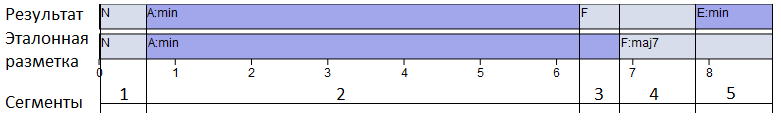
\includegraphics [scale=0.80] {EvaluationSegments}
  \caption{Сопоставление последовательностей аккордов.}
  \label{img:evaluation_segments}  
\end{figure}

Пусть заданы 2 последовательности аккордов: правильная и определённая при помощи
алгоритма. Объединим множества границ аккордов из обоих последовательностей в
одно множество. Используя эти границы, разделим исходную композицию на
сегменты (как на рисунке \ref{img:evaluation_segments}), на каждом из которых
однозначно заданы правильный аккорд $c_{ref}$ и определённый автоматически
$c_{est}$. Пусть также $c_{ref} \in C_{REF}$ -- множество всех аккордов,
встречающихся в аннотациях, а $c_{est} \in C_{EST}$ -- множество всех аккордов,
которые могут быть результатом распознавания при помощи данного алгоритма.

Практически всегда $C_{EST} \subset C_{REF}$, поэтому возникает вопрос о том,
как сопоставлять фрагменты, на которых $c_{ref} \not \in C_{EST}$. Такие
фрагменты можно либо отбрасывать, либо задать сюръективное отображение
$\mathcal{M}: C_{MI} \to C_{MO}$, которое <<сложным>> аккордам из множества
$C_{MI}$ будет сопоставлять <<простые>> аккорды из множества $C_{MO}$. Нужно
выбрать эти множества и отображение $\mathcal{M}$ таким образом, чтобы $C_{EST}
\subset C_{MI}$. Сравниваться при этом будут аккорды $\mathcal{M}(c_{ref})$ и
$\mathcal{M}(c_{est})$. Сегменты, на которых $c_{ref} \not \in C_{MI}$,
отбрасываются. Примером отображения $\mathcal{M}$ может служить отображение,
которое всем аккордам, состоящим из мажорного трезвучия и более высоких ступеней
(например, доминантсептаккорд, нонаккорды и другие) сопоставляет мажорный
аккорд, соответствующий этому трезвучию.

Если необходимо оценить качество распознавания аккордов определенного типа
(например, только трезвучий или только мажорных аккордов), можно ввести
дополнительные множества $C_{LI}$ и $C_{LO}$, ограничивающие соответственно
множества $C_{MI}$ и $C_{MO}$. Тогда аккорды $(c_{ref}, c_{est})$ сравниваются
(не отбрасываются), только если $c_{ref} \in C_{LI} \cap C_{MI}$ и
$\mathcal{M}(c_{ref}) \in \mathcal{M}(C_{LI} \cap C_{MI}) \cap C_{LO}$.

Пусть $\mathcal{S}:C_{SR} \times C_{SE} \to \mathbb{R}^+$ -- функция оценки,
причем $\mathcal{M}(C_{LI} \cap C_{MI}) \cap C_{LO} \subset C_{SR}$ и $C_{MO}
\subset C_{SE}$. Эта функция сопоставляет паре аккордов $\mathcal{M}(c_{ref})$ и
$\mathcal{M}(c_{est})$ неотрицательное действительное число, которое выражает
сходство этих аккордов между собой. Например, можно определить функцию
$\mathcal{S}$ как равную 1 в случае, когда аккорды совпадают, и 0 иначе.

Как видно из \cite{Pauwels2013}, полученные цифры сильно различаются в
зависимости от выбора отображения $\mathcal{M}$ и функции оценки $\mathcal{S}$,
и даже в зависимости от некоторых мелких деталей, таких как способ
синтаксического разбора названий аккордов. Не всегда в статьях корректно
указываются использованные метрики, что делает затруднительным непосредственное
сравнение оценок качества распознавания из статей друг с другом. В этом состоит
главная ценность соревнования MIREX Audio Chord Estimation, где гарантированно
используются одни и те же коллекции и метрики для оценки всех алгоритмов.

Рассмотрим 3 наиболее характерных метрики из \cite{Pauwels2013}.

\begin{enumerate}
  \item ``Mirex2010''. В ней не используется отображение $\mathcal{M}$, а
  функция оценки $\mathcal{S}$ строится следующим образом. Сначала $c_{ref}$ и
  $c_{est}$ преобразуются в множества тональных классов, для которых находится
  пересечение. Обозначим количество элементов в пересечении за $u$.
  $\mathcal{S}=1$ в случаях:
  \begin{itemize}
    \item $c_{ref}$ является уменьшенным или увеличенным аккордом и $u \geq 2$;
    \item $c_{ref}$ и $c_{est}$ являются символами отсутствия аккорда;
    \item $u \geq 3$.
  \end{itemize}
  В остальных случаях $\mathcal{S}=0$, то есть $\mathcal{S}:C_{SR} \times C_{SE}
  \to \{0, 1\}$. 
  \item ``Triads''. Отображение $\mathcal{M}$ строится следующим образом. Если
  существует мажорное или минорное трезвучие с основной нотой, соответствующей
  основной ноте аккорда, и имеющее 3 общих ноты с аккордом, то оно
  сопоставляется этому аккорду. Например, для доминантсептаккорда с добавленной
  ступенью G:7(9) результатом сопоставления будет мажорное трезвучие G:maj, а
  для аккорда F:aug сопоставления не существует. Аккорды, которым невозможно
  сопоставить мажорное или минорное трезвучие, из оценки исключаются.
  $\mathcal{S}=1$ тогда и только тогда, когда $c_{ref}$ и $c_{est}$ совпадают.
  \item ``Tetrads''. Отображение $\mathcal{M}$ строится аналогично ``Triads'',
  но помимо мажорного и минорного трезвучий рассматриваются также мажорный и
  минорный септаккорды и доминантсептаккорд, а в качестве результата выбирается
  аккорд, имеющий наибольшее количество общих нот с заданным. Так, для
  доминантсептаккорда с добавленной ступенью G:7(9) результатом сопоставления
  будет доминантсептаккорд G:7. $\mathcal{S}=1$ тогда и только тогда, когда
  $c_{ref}$ и $c_{est}$ совпадают.
\end{enumerate}

Отметим, что при использовании метрики ``Mirex2010'' ни один сегмент не
отбрасывается. Это может быть нежелательно, поскольку в полученном результате
будут учитываться в том числе и сегменты, содержащие аккорды, которые в принципе
не могут быть распознаны имеющимся методом. Ещё одним недостатком этой метрики
является невозможность различить трезвучие и содержащий его септаккорд: при
совпадении хотя бы трёх нот аккорды будут считаться совпадающими. Поэтому в
дальнейших экспериментах будут использоваться метрики ``Triads'' и ``Tetrads'',
позволяющие более точно оценить качество распознавания аккордов. Первая метрика
будет использоваться вместе с набором из 24 шаблонов для всех мажорных и
минорных трезвучий, а вторая -- с набором из 60 шаблонов, в который входят также
шаблоны для всех доминантсептаккордов и мажорных и минорных септаккордов.

Метрика ``Mirex2010'' использовалась в соревновании MIREX Audio Chord Estimation
в 2010, 2011 и 2012 годах. Но в 2013 году вместо неё были использованы метрики
``Triads'', ``Tetrads'', а также некоторые другие, позволяющие учесть также
обращения аккордов и басовую ноту. Поскольку описываемый здесь алгоритм не
предназначен для определения обращений аккордов, нет смысла использовать эти
дополнительные метрики.

Обозначим за $\ell_1, \ell_2, \ldots, \ell_{N_{segm}}$ длины всех сегментов в
пределах одной композиции, а $s_1, s_2, \ldots, s_{N_{segm}}$ -- соответствующие
значения метрики. Тогда \emph{коэффициент перекрытия (overlap ratio, OR)} для
данной композции определяется как
\begin{equation} \label{eq:or}
OR = \frac{\sum_{i=1}^{N_{segm}} s_i \ell_i}{\sum_{i=1}^{N_{segm}} \ell_i}
\end{equation}
При этом неважно, были ли ceгменты взяты из одной и той же композиции или из
нескольких разных. Но для того, чтобы иметь возможность определить
статистически значимые различия между системами, в экспериментах будем
определять коэффициент перекрытия отдельно для каждой композиции.

Для примера, на рисунке \ref{img:evaluation_segments} $s_1 = s_2 = s_4 = 1$,
$s_3 = s_5 = 0$. На сегментах 1 и 2 аккорды совпадают, на сегменте 4 аккорды
F:maj и F:maj7 имеют 3 общих ступени F, A, C.

Пусть коллекция содержит $N_{tracks}$ композиций, для каждой из которых
вычислен коэффициент перекрытия $OR_k$. Обозначим за $L_i =
\sum_{i=j}^{N_{segm}} \ell_j$ длину $i$-й композиции. Тогда совокупная метрика
для коллекции, называемая \emph{взвешенным средним коэффициентом перекрытия
(weighted average overlap ratio, WAOR)}, вычисляется следующим образом:
\begin{equation} \label{eq:waor}
WAOR = \frac{\sum_{i=1}^{N_{tracks}} OR_i \cdot L_i}{\sum_{i=1}^{N_{tracks}}
L_i}
\end{equation}
Такой же способ усреднения применяется в соревнованиях MIREX Audio Chord
Estimation. В качестве результатов экспериментов в последующих разделах
приведены значения взвешенных средних коэффициентов перекрытия для метрик
``Triads'' и ``Tetrads''.

\subsection{Сопоставление границ сегментов}

Метрика для сопоставления границ сегментов была введена Маухом в
\cite{MauchThesis2010}. Начиная с 2013 года она также применяется в
соревнованиях MIREX Audio Chord Estimation. Она позволяет оценить качество
определения границ аккордов алгоритмом, игнорируя при этом сами названия
аккордов.

Пусть заданы 2 разбиения звукозаписи длины $L$ на сегменты $G^0 = (G_i^0)$ и $G
= (G_i)$. Направленное расхождение Хэмминга определяется как:
$$
h(G||G^0) = \sum_{i=1}^{N_G} \left( |G_i^0| - \underset{j}{\operatorname{max}}
|G_i^0 \cap G_j| \right)
$$
где $N_G$ -- количество сегментов в разбиении $G$, а $| \cdot |$ -- длина
сегмента. Оно определяет, насколько $G$ фрагментировано по отношению к $G^0$.
Тогда \emph{сегментация} $H(G, G^0)$ определяется как
$$H(G, G^0) = 1 - \frac{1}{L} max\{ h(G||G^0), h(G^0||G) \} \in [0,1]$$

В экспериментах одно из разбиений задаётся правильной разметкой звукозаписи, а
другое -- результатом распознавания аккордов с использованием только шаблонов
для мажорных и минорных трезвучий. Для усреднения значений сегментации
вычислялось простое среднее арифметическое от полученных значений по всем
композициям из коллекции.

\subsection{Статистическая значимость}

При сравнении нескольких вариантов алгоритма помимо средних значений метрик
качества необходимо понять, действительно ли между этими вариантами имеются
статистически значимые различия. Для проверки этого предположения будем
использовать непараметрический критерий Фридмана. Он позволяет проверять
гипотезы о различии более двух зависимых выборок. В отличие от дисперсионного
анализа (ANOVA), критерий Фридмана не требует предположений о нормальности
распределения значений метрик для разных композиций, а также одинаковых
дисперсий этих распределений для разных вариантов алгоритма (как отмечается в
\cite{Mauch2010}, эти предположения не является верными в данном случае).

Однако, если в соответствии с критерием Фридмана удаётся отвергнуть нулевую
гипотезу (об отсутствии различий между разными методами), необходимо выяснить,
для каких пар методов имеется статистически значимая разница в качестве
распознавания аккордов. Для этого вычисляется среднее Тьюки (Tukey's honestly
significant difference). В отличие от T-теста, при его допускаются множественные
попарные сравнения. Этот метод используется для сравнения качества работы разных
алгоритмов в рамках всех соревнований MIREX \cite{Downie2008}. В экспериментах
среднее Тьюки вычислялось для значений взвешенного среднего перекрытия,
полученных с использованием метрики ``Triads''.

\subsection{Совокупная длительность}

Совокупная длительность композиций в коллекции составляет 61701,61 с. Совокупная
длительность участвующих в оценке фрагментов (для аккордов на которых определено
отображение $\mathcal{M}$) составляет 58937,75 с, что составляет более 95\% от
совокупной длительности всех композиций.

Совокупная продолжительность звучания аккордов каждого из типов (с учётом
отображения $\mathcal{M}$ для метрик) приведена в таблице \ref{Tchord_stat}.
Видно, что в звукозаписях из коллекции преобладают мажорные трезвучия и аккорды,
основанные на них.

\begin{table} [htbp]
  \centering
  \parbox{15cm}{\caption{Совокупная продолжительность звучания аккордов в
  секундах}
  \label{Tchord_stat}}
  \begin{tabular}{|l||l|l||l|l|}
  \hline
  Тип & Triads & \% & Tetrads & \% \\
  \hline
  maj & 41733.38 & 70.81\% & 34381.76 & 58.34\% \\
  7 & - & - & 4862.02 & 8.25\% \\
  maj7 & - & - & 2489.6 & 4.22\% \\
  \hline
  min & 14681.45 & 24.91\% & 9921,61 & 16.83\% \\
  min7 & - & - & 4759.83 & 8.08\% \\
  \hline
  N & 2522.92 & 4.28\% & 2522.92 & 4.28\% \\
  \hline
  \end{tabular}
\end{table}

\subsection{Типы ошибок}

Для удобства в дальнейшем ошибки будут сгруппированы по типам. Название типа
ошибок начинается с типа ожидаемого (правильного) аккорда и может включать тип
неправильно определённого аккорда, например, maj или maj-min. Ошибки maj-maj
соответствуют случаю, когда вместо мажорного аккорда был определён мажорный
аккорд с другой основной нотой. Поскольку используемые метрики ``Triads'' и
``Tetrads'' используют отображение $\mathcal{M}$ для сведения в некотором
смысле более сложных аккордов к более простым (например, G:7(9) к G:7 или
G:maj), это же отображение будет применяться ко всем ожидаемым аккордам для
уменьшения количества типов ошибок. Так, при использовании метрики ``Triads''
тип maj7-min будет включен в тип maj-min и не будет рассматриваться отдельно.
Аккорды, которым в результате действия отображения $\mathcal{M}$ не
сопоставляется никакой другой аккорд, исключаются как из итогового результата,
так и из статистики ошибок. Типы ошибок N-chord и chord-N (где chord -- любой
аккорд) будем объединять в один, поскольку на них оказывает влияние в первую
очередь способ определения отсутствия звучащего аккорда.

Ошибки метода можно рассматривать на трёх уровнях. Каждый последующий уровень
уточняет предыдущий.
\begin{enumerate}
 \item Совокупная длительность ошибочных фрагментов в зависимости от типа
 звучащего аккорда. Например, maj.
 \item Совокупная длительность ошибочных фрагментов в зависимости от типа
 звучащего аккорда и типа неверно определённого аккорда. Например, maj-min.
 Тип maj-maj соответствует случаям, когда вместо мажорного аккорда неверно
 определён мажорный аккорд с другим основным звуком.
 \item Совокупная длительность ошибочных фрагментов в зависимости от типа
 звучащего аккорда, типа неверно определённого аккорда и расстояния в полутонах
 между основными звуками аккордов.
\end{enumerate}

В дальнейшем на диаграммах под буквами а), б) будет показано распределение
ошибок, соответствующее первому уровню. Под буквами в), г) (если
присутствуют) -- соответствующее второму или третьему уровню. Высота столбцов
соответствует совокупной длительности фрагментов звукозаписей, содержащих ошибки
соответствующего типа. Столбцы сгруппированы по типам ошибок. Цвета столбцов
соответствуют разным значениям описываемого параметра.

\section{Вычисление спектрограммы} \label{sect3_spectcalc}

На данном этапе необходимо выбрать наилучшие из доступных алгоритмов для
определения ритма и определения частоты настройки. Наилучшее значение
для параметра $d$, задающего задержку для моментов времени, в которых
анализируется спектр звука, относительно моментов начала метрических долей,
также должно быть определено на этом этапе. Кроме того, необходимо определить
наилучшие значения для параметров преобразования постоянного качества:
разрешение по частоте $N_0$ (количество компонент, приходящихся на октаву) и
количество октав $N / N_0$, а также для количества вставляемых промежуточных
столбцов спектрограммы $T$ и размера окна при сглаживании $w$.

\subsection{Определение ритма} \label{ssect3_beattrack}

Были рассмотрены 3 алгоритма, позволяющие определить моменты начала метрических
долей в звукозаписи: \emph{BeatRoot} \cite{Dixon2007}, \emph{Beat tracker} от
Дэвиса \cite{Davies2007} (\emph{DBT}) из набора плагинов \emph{Queen Mary Vamp
plugins}\footnote{\url{http://www.isophonics.net/QMVampPlugins}} для системы
извлечения музыкальной информации из музыкальных файлов
\emph{Vamp}\footnote{\url{http://www.vamp-plugins.org/}} и плагина \emph{INESC
Porto Beat Tracking plugin} \cite{Oliveira2012} (\emph{IBT}) для этой же
системы. Выбор алгоритмов обусловлен наличием свободно доступной реализации.
\emph{BeatRoot} дополнительно потребовал небольшого вмешательства в исходный
код для уменьшения потребления вычислительных ресурсов. Кроме того, на 6
композициях из анализруемого набора этот алгоритм не смог определить ритм,
поэтому для этих композиций использовались значения, полученные при помощи DBT.
Для всех алгоритмов определения ритма использовалось значение задержки $d=100$
мс.

\begin{table} [htbp]
  \centering
  \parbox{15cm}{\caption{Влияние алгоритма определения ритма на
  качество распознавания аккордов} \label{TBT}}
%  \begin{center}
  \begin{tabular}{|l|l|l|l|}
  \hline
  Алгоритм & Triads & Tetrads & Сегментация \\
  \hline
  BeatRoot + DBT & 0.7720 & 0.4310 & 0.8141 \\
  DBT & 0.7592 & 0.4401 & 0.8007 \\
  IBT & 0.7335 & 0.4160 & 0.7635 \\
  -- & 0.7113 & 0.4550 & 0.7584 \\
  \hline
  \end{tabular}
%  \end{center}
\end{table}

\begin{figure}[htbp]
  \begin{minipage}[h]{0.49\linewidth}
    \center{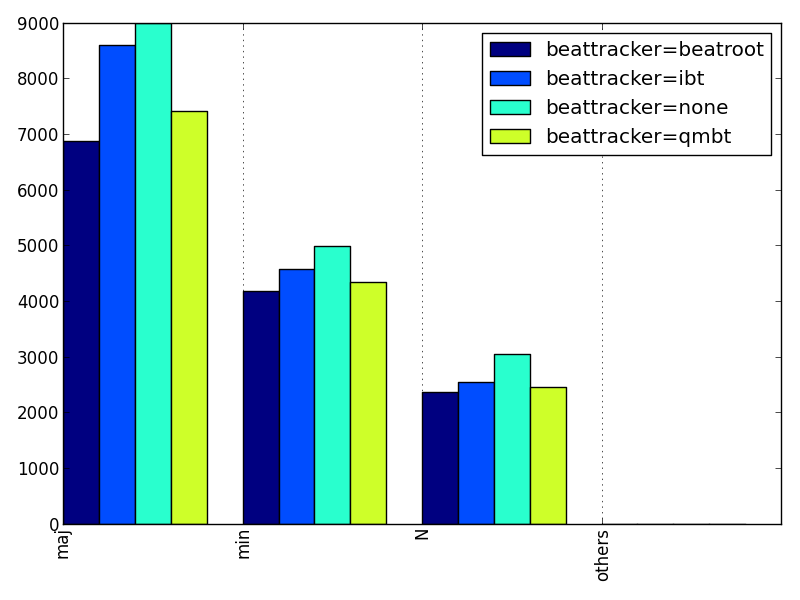
\includegraphics[scale=0.38]{errors/beattracker3a} \\ а)}
  \end{minipage}
  \hfill
  \begin{minipage}[h]{0.49\linewidth}
    \center{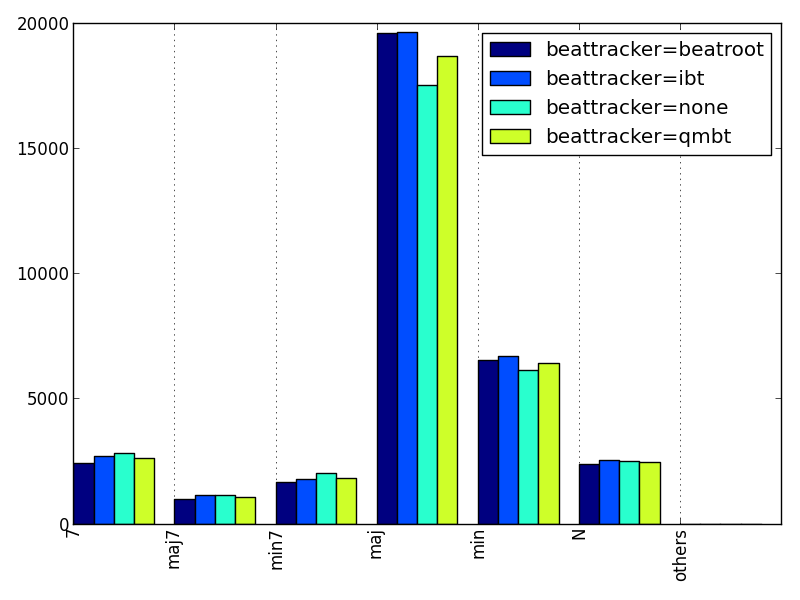
\includegraphics[scale=0.38]{errors/beattracker4a} \\ б)}
  \end{minipage}
  \caption{Диаграмма ошибок для разных методов определения ритма}
  \label{img:beattracker}
\end{figure}

Наилучшие полученные для данных алгоритмов результаты показаны в таблице
\ref{TBT}. \emph{BeatRoot} показал наилучший результат, статистически значимо
превосходящий результаты, полученные с использованием алгоритмов \emph{IBT} и
\emph{DBT}. Это достаточно удивительно, поскольку первая версия алгоритма
\emph{BeatRoot} была представлена ещё в 2001 году, а в данной работе
использовалась его исправленная версия от 2007 года. При этом \emph{DBT} был
представлен в 2007 году, а \emph{IBT}, схожий по принципу работы с
\emph{BeatRoot}, -- в 2012 году. 

Последняя строка в таблице \ref{TBT} показывает результат, полученный без
определения ритма. При этом искусственно генерировалась последовательность
значений времени с шагом в 0.5 с, которые считались моментами начала метрических
долей, с задержкой $d=0$ мс. Ожидаемо, это привело к наихудшему результату,
статистически значимо отличающемуся от остальных.

\subsection{Определение задержки} \label{ssec3_offset}

\begin{table} [htbp]
  \centering
  \parbox{15cm}{\caption{Влияние задержки относительно моментов начала
  метрических долей на качество распознавания аккордов} \label{TDelay}}
  \begin{tabular}{|l|l|l|l|}
  \hline
  $d$ & Triads & Tetrads & Сегментация \\
  \hline
  0 мс & 0.7558 & 0.4351 & 0.7932 \\
  60 мс & 0.7689 & 0.4303 & 0.8096 \\
  80 мс & 0.7711 & 0.4290 & 0.8123 \\
  100 мс & 0.7720 & 0.4310 & 0.8141 \\
  120 мс & 0.7724 & 0.4374 & 0.8144 \\
  \hline
  \end{tabular}
\end{table}

\begin{figure}[htbp]
  \begin{minipage}[h]{0.49\linewidth}
    \center{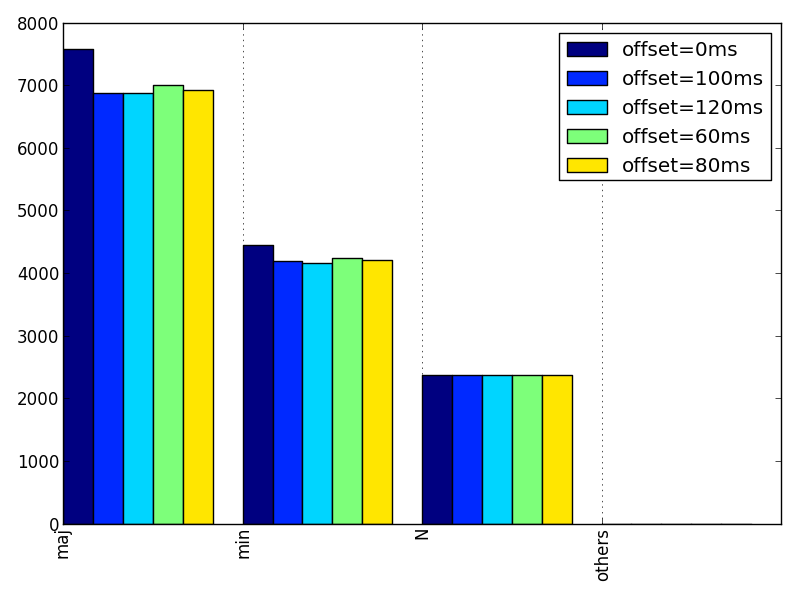
\includegraphics[scale=0.38]{errors/offset3a} \\ а)}
  \end{minipage}
  \hfill
  \begin{minipage}[h]{0.49\linewidth}
    \center{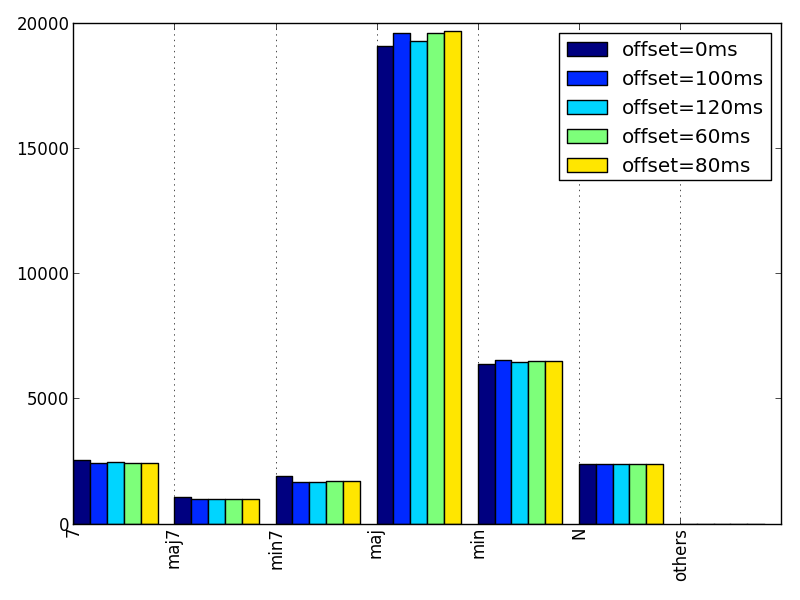
\includegraphics[scale=0.38]{errors/offset4a} \\ б)}
  \end{minipage}
  \hfill
  \begin{minipage}[h]{0.49\linewidth}
    \center{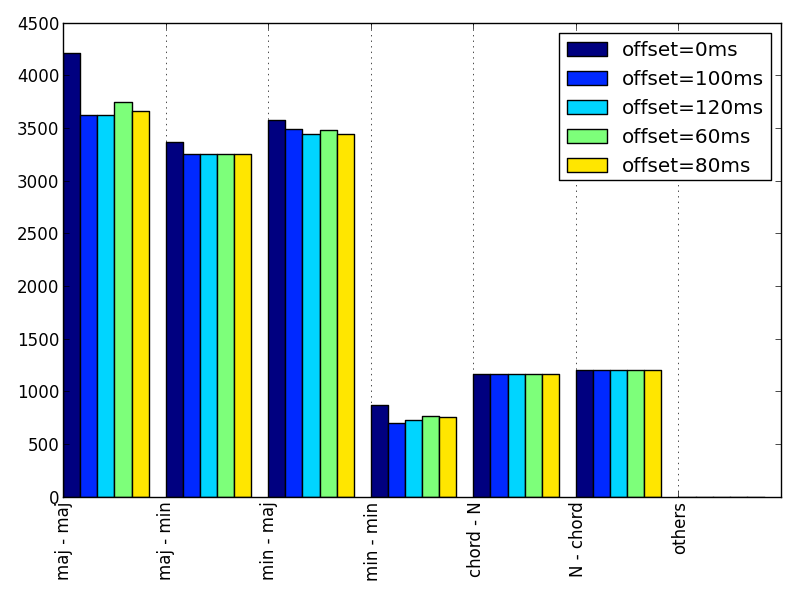
\includegraphics[scale=0.38]{errors/offset3} \\ в)}
  \end{minipage}
  \hfill
  \begin{minipage}[h]{0.49\linewidth}
    \center{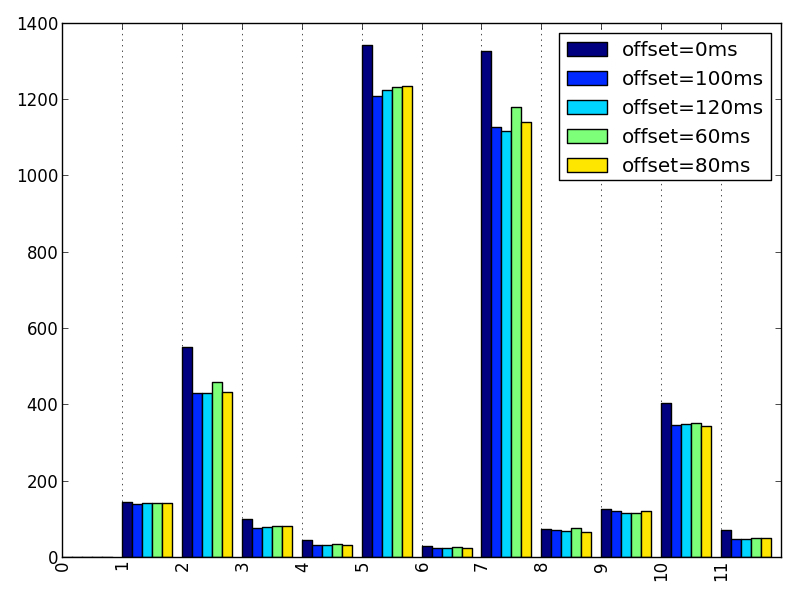
\includegraphics[scale=0.38]{errors/offset_maj_-_maj} \\ г)}
  \end{minipage}
  \caption{Диаграмма ошибок для разных значений $d$}
  \label{img:offset}
\end{figure}

Любое из использованных значений задержки от 60 мс до 120 мс приводит к
статистически значимому улучшению качества распознавания аккордов по сравнению
с отсутствием задержки. При этом варианты с ненулевыми значениями задержки не
имеют статистически значимых различий. Как видно из рисунка \ref{img:offset} в),
в случае определения только трезвучий при нулевой задержке ухудшение качества
распознавания вызвано в основном ошибочным определением основной ноты, а не
типа аккорда. Рисунок \ref{img:offset} г) показывает распределение расстояний
между основными звуками аккордов в полутонах для случая maj-maj. Расстояния в 5
и 7 полутонов соответствуют случаям, когда основной звук правильного аккорда
является квинтой ошибочного и наоборот.

\subsection{Определение частоты настройки} \label{ssec3_tunfreq}

Были проведены эксперименты по распознаванию аккордов с использованием
описанного в разделе \ref{ssect1_f0} алгоритма для вычисления частоты настройки
со следующими значениями параметров:
\begin{itemize}
  \item $f_{min} = 220$ Гц, $N_0 = 12 \cdot 10 = 120$ компонент на октаву;
  \item $f_{min} = 440$ Гц, $N_0 = 12 \cdot 10 = 120$ компонент на октаву.
\end{itemize}
Охват во всех случаях составлял 4 октавы. Также для сравнения были проведены
эксперименты без коррекции частоты настройки и с использованием алгоритма,
описанного Маухом в \cite{MauchThesis2010}, раздел 3.1.3 и реализованного в виде
плагина для системы \emph{Vamp}.

\begin{table} [htbp]
  \centering
  \parbox{15cm}{\caption{Влияние алгоритма определения частоты настройки на
  качество распознавания аккордов} \label{TTunFreq}}
  \begin{tabular}{|l|l|l|l|}
  \hline
  Алгоритм & Triads & Tetrads & Сегментация \\
  \hline
  $f_{min} = 220$ Гц & 0.7720 & 0.4310 & 0.8141 \\
  $f_{min} = 440$ Гц & 0.7719 & 0.4263 & 0.8134 \\
  Маух \cite{MauchThesis2010} & 0.7718 & 0.4382 & 0.8142 \\
  -- & 0.7657 & 0.4107 & 0.8120 \\
  \hline
  \end{tabular}
\end{table}

\begin{figure}[h]
  \begin{minipage}[h]{0.49\linewidth}
    \center{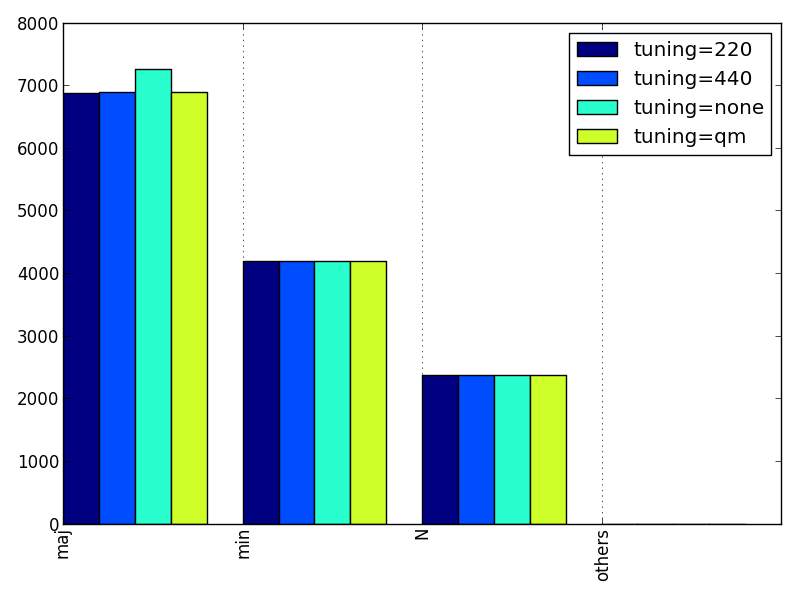
\includegraphics[scale=0.38]{errors/tuning3a} \\ а)}
  \end{minipage}
  \hfill
  \begin{minipage}[h]{0.49\linewidth}
    \center{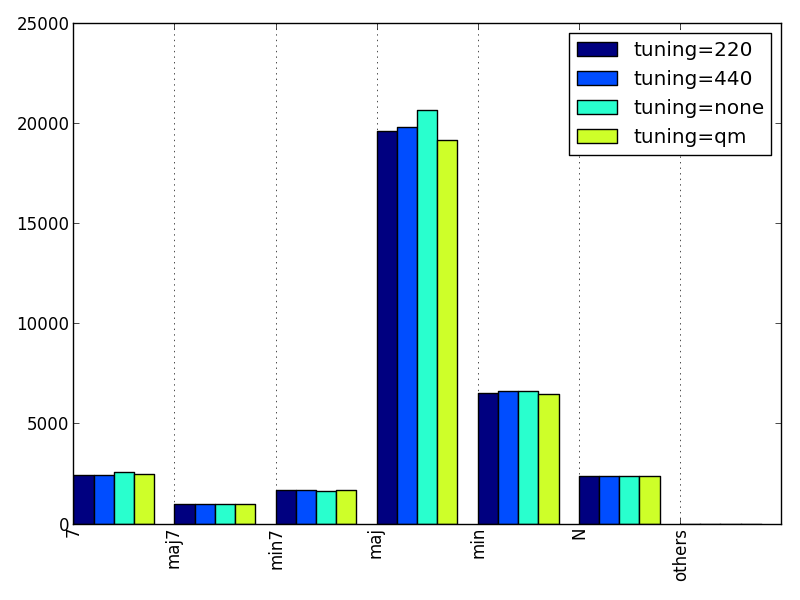
\includegraphics[scale=0.38]{errors/tuning4a} \\ б)}
  \end{minipage}
  \hfill
  \begin{minipage}[h]{0.49\linewidth}
    \center{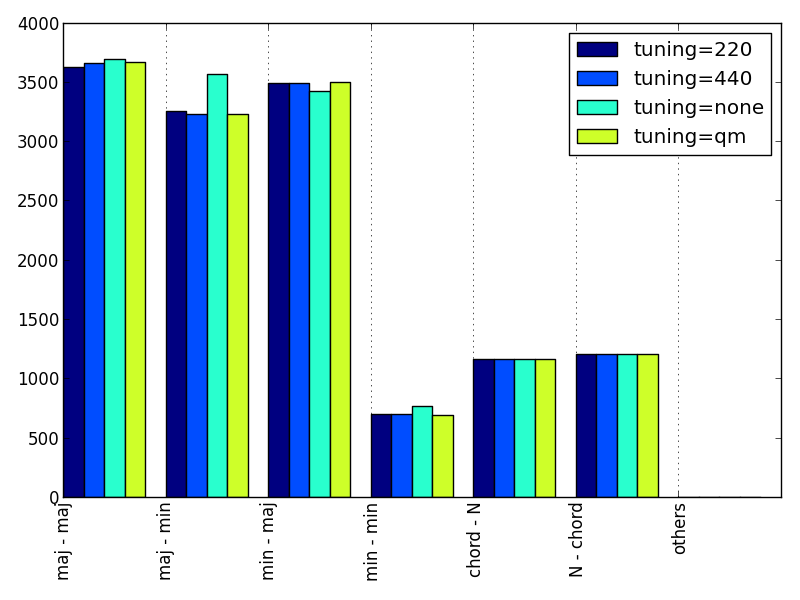
\includegraphics[scale=0.38]{errors/tuning3} \\ в)}
  \end{minipage}
  \hfill
  \begin{minipage}[h]{0.49\linewidth}
    \center{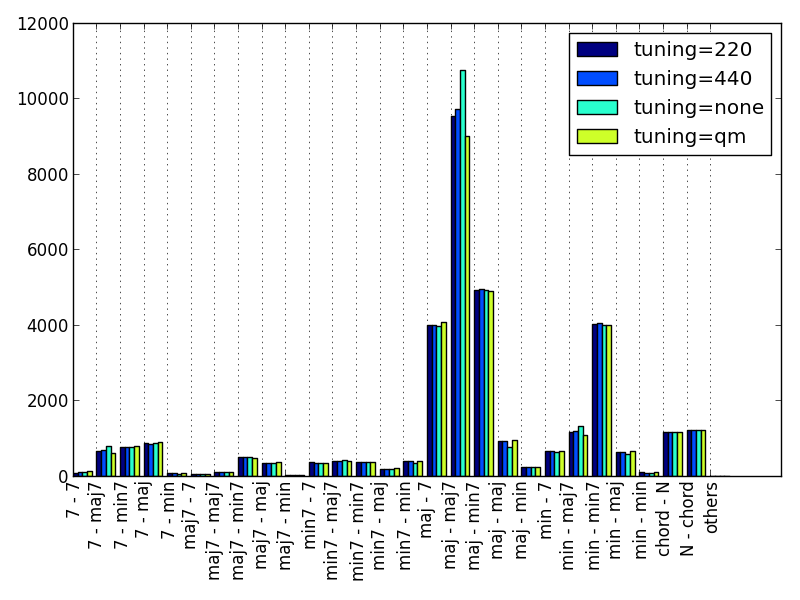
\includegraphics[scale=0.38]{errors/tuning4} \\ г)}
  \end{minipage}
  \caption{Диаграмма ошибок для разных методов определения частоты настройки}
  \label{img:tuning}
\end{figure}

Результаты экспериментов приведены в таблице \ref{TTunFreq}. Как видно,
определение частоты настройки приводит к улучшению качества распознавания
аккордов, которое, однако, не является статистически значимым ни для одного из
алгоритмов. Из рисунка \ref{img:tuning} в) можно заметить, что определение
частоты настройки помогает уменьшить количество ошибочных определений минорного
аккорда для случая трезвучий. А рисунок \ref{img:tuning} г) показывает, что для
случая септаккордов оно помогает уменьшить количество ошибочных определений
мажорного септаккорда.

\subsection{Разрешение по времени и по частоте, сглаживание} \label{ssect3_Tw}

Вставка между каждыми двумя соседними моментами начала метрических долей
$T-1$ промежуточных значений позволяет повысить разрешение спектрограммы по
времени. Затем, после применения скользящего медианного фильтра с размером окна
$w$ и прореживания в $T$ раз, спектрограмма содержит ровно 1 столбец на каждую
метрическую долю. Ясно, что при больших значениях $T$ имеет смысл выбирать
больше значения $w$ и наоборот. В таблице \ref{TTw} приведены значения для
некоторых комбинаций $T$ и $w$.

\begin{table} [htbp]
  \centering
  \parbox{15cm}{\caption{Влияние параметров $T$ и $w$ на качество распознавания
  аккордов} \label{TTw}}
  \begin{tabular}{|l|l|l|l|}
  \hline
  Значения параметров & Triads & Tetrads & Сегментация \\
  \hline
  $T = 2$, $w = 1$ & 0.7334 & 0.3670 & 0.7999 \\
  $T = 2$, $w = 3$ & 0.7537 & 0.4200 & 0.8094 \\
  $T = 2$, $w = 5$ & 0.7672 & 0.4501 & 0.8149 \\
  \hline
  $T = 4$, $w = 3$ & 0.7624 & 0.4621 & 0.8115 \\
  $T = 4$, $w = 5$ & 0.7619 & 0.4440 & 0.7992 \\
  $T = 4$, $w = 7$ & 0.7425 & 0.3909 & 0.7664 \\
  $T = 4$, $w = 9$ & 0.7194 & 0.3583 & 0.7307 \\
  $T = 4$, $w = 11$ & 0.6913 & 0.3197 & 0.6917 \\
  \hline
  $T = 8$, $w = 11$ & 0.7715 & 0.4464 & 0.8176 \\
  $T = 8$, $w = 13$ & 0.7720 & 0.4364 & 0.8160 \\
  $T = 8$, $w = 15$ & 0.7720 & 0.4310 & 0.8141 \\
  $T = 8$, $w = 17$ & 0.7707 & 0.4273 & 0.8089 \\
  $T = 8$, $w = 19$ & 0.7696 & 0.3923 & 0.8043 \\
  \hline
  \end{tabular}
\end{table}

\begin{figure}[htbp]
  \begin{minipage}[h]{0.49\linewidth}
    \center{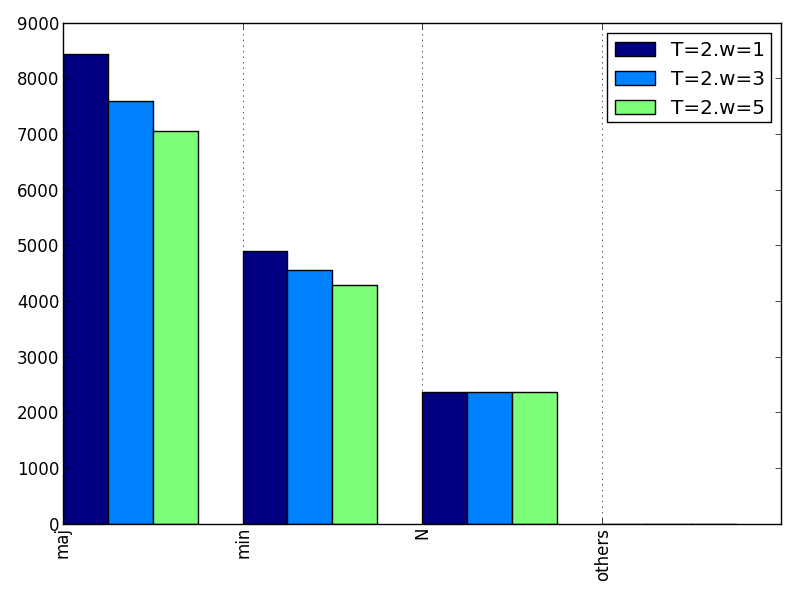
\includegraphics[scale=0.38]{errors/T=2w3a} \\ а)}
  \end{minipage}
  \hfill
  \begin{minipage}[h]{0.49\linewidth}
    \center{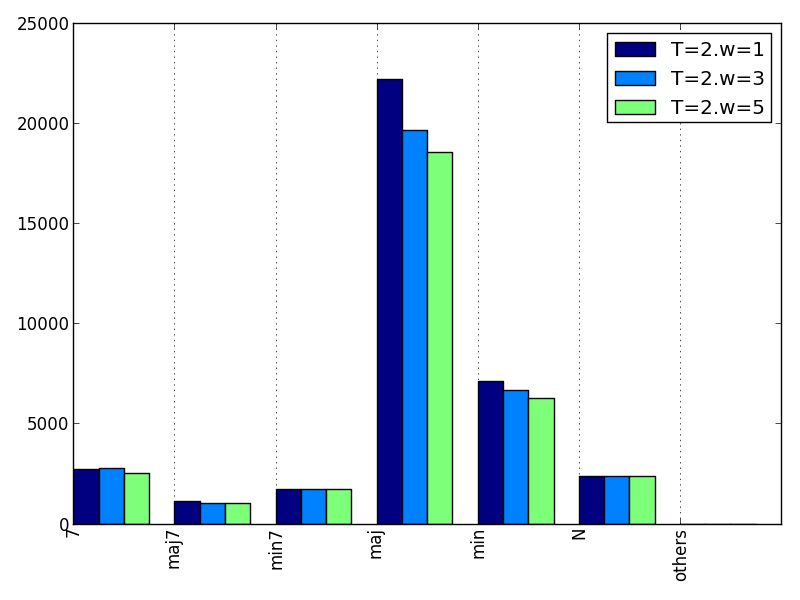
\includegraphics[scale=0.38]{errors/T=2w4a} \\ б)}
  \end{minipage}
  \caption{Диаграмма ошибок для разных значений $w$ при $T=2$}
  \label{img:T2}
\end{figure}

\begin{figure}[htbp]
  \begin{minipage}[h]{0.49\linewidth}
    \center{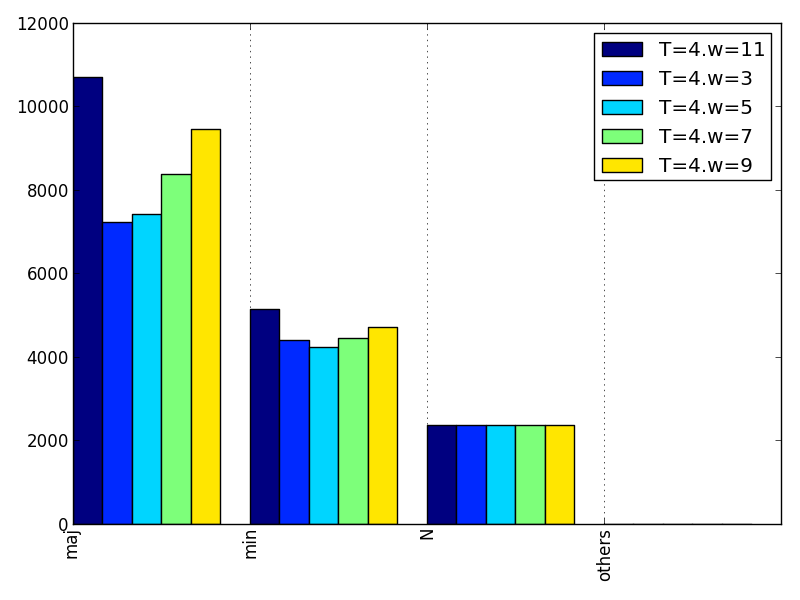
\includegraphics[scale=0.38]{errors/T=4w3a} \\ а)}
  \end{minipage}
  \hfill
  \begin{minipage}[h]{0.49\linewidth}
    \center{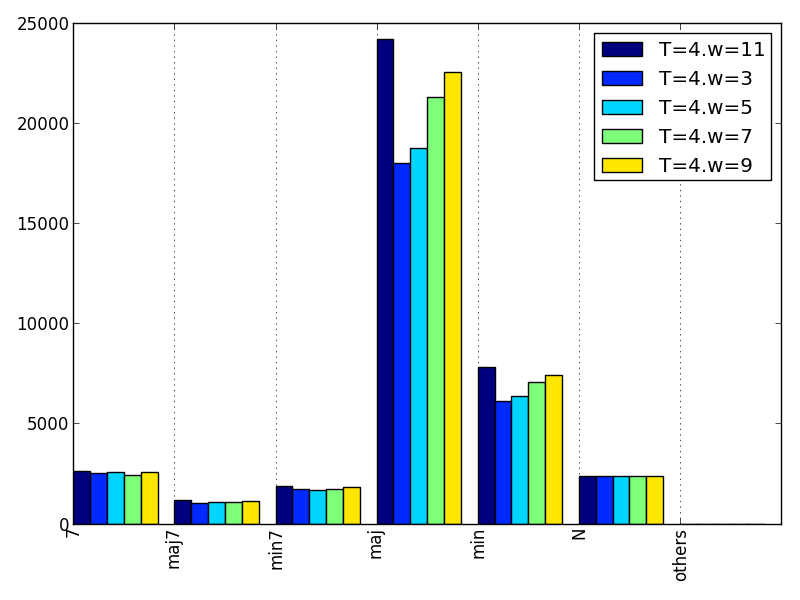
\includegraphics[scale=0.38]{errors/T=4w4a} \\ б)}
  \end{minipage}
  \caption{Диаграмма ошибок для разных значений $w$ при $T=4$}
  \label{img:T4}
\end{figure}

\begin{figure}[htbp]
  \begin{minipage}[h]{0.49\linewidth}
    \center{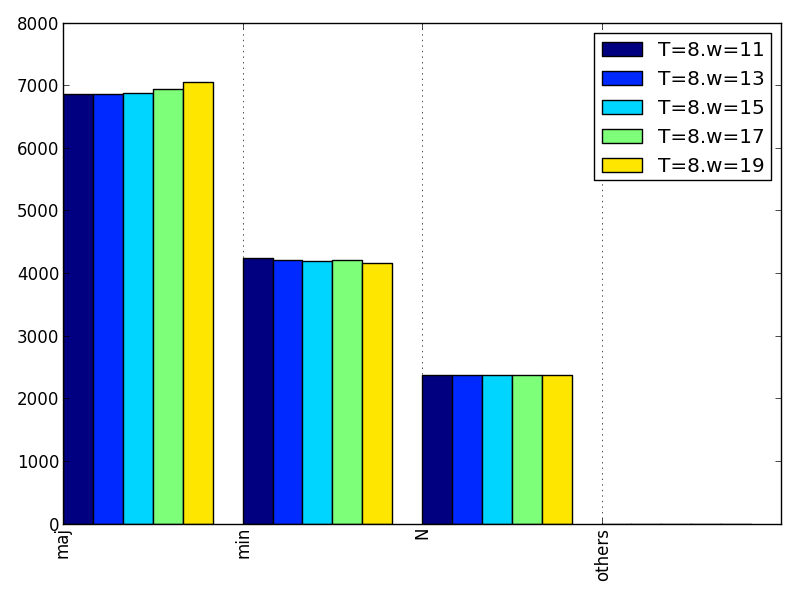
\includegraphics[scale=0.38]{errors/T=8w3a} \\ а)}
  \end{minipage}
  \hfill
  \begin{minipage}[h]{0.49\linewidth}
    \center{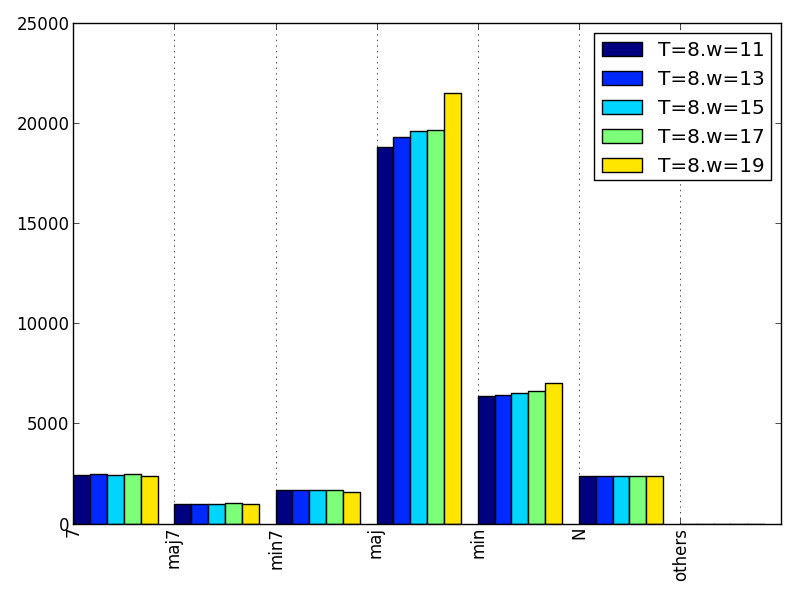
\includegraphics[scale=0.38]{errors/T=8w4a} \\ б)}
  \end{minipage}
  \caption{Диаграмма ошибок для разных значений $w$ при $T=8$}
  \label{img:T8}
\end{figure}

При $T=2$ качество распознавания аккордов существенно хуже для случая $w=1$, что
фактически соответствует отказу от добавления промежуточных значений и
последующих сглаживания и прореживания. Все различия между результатами
статистически значимы.

При $T=4$ результат существенно ухудшается с ростом размера окна $w$ Наилучшие
результаты получены при $w=3$ и $w=5$, и они статистически значимо превосходят
остальные.

При $T=8$ разница между всеми вариантами очень невелика, статистически значимых
различий не обнаружено.

Как показывают рисунки \ref{img:T2}, \ref{img:T4}, \ref{img:T8}, разные значения
$w$ влияют только на количество ошибок при распознавании мажорных и минорных
трезвучий, но не на количество ошибок при распознавании септаккордов.

% Отдельно было проведено сравнение наилучших вариантов для каждого значения $T$.
% Между вариантами $T=4, w=7$ и $T=8, w=15$ нет статистически значимой разницы в
% качестве распознавания аккордов; разница в абсолютных значениях метрик также
% незначительна. При $T=2, w=3$ результат статистически значимо хуже двух других.
% 
% Интересно, что наилучшие результаты достигаются при $w = 2T-1$, что для каждого
% момента времени исходной последовательности соответствует фильтрации по
% значениям спектра, вычисленным в этот момент и в $T-1$ добавленных промежуточных
% точках справа и слева. Из этого эксперимента видно, что увеличение разрешения по
% времени для последовательности моментов начала метрических долей по крайней мере
% в 4 раза приводит к заметному улучшению качества распознавания аккордов.

\begin{table} [htbp]
  \centering
  \parbox{15cm}{\caption{Влияние параметра $N_0$ на качество распознавания
  аккордов} \label{TN0}}
  \begin{tabular}{|l|l|l|l|}
  \hline
  Значения $N_0$ & Triads & Tetrads & Сегментация \\
  \hline
  $N_0 = 12$ & 0.6418 & 0.0632 & 0.7898 \\
  $N_0 = 36$ & 0.7720 & 0.4310 & 0.8141 \\
  $N_0 = 60$ & 0.7746 & 0.4266 & 0.8083 \\
  \hline
  \end{tabular}
\end{table}

\begin{figure}[htbp]
  \begin{minipage}[h]{0.49\linewidth}
    \center{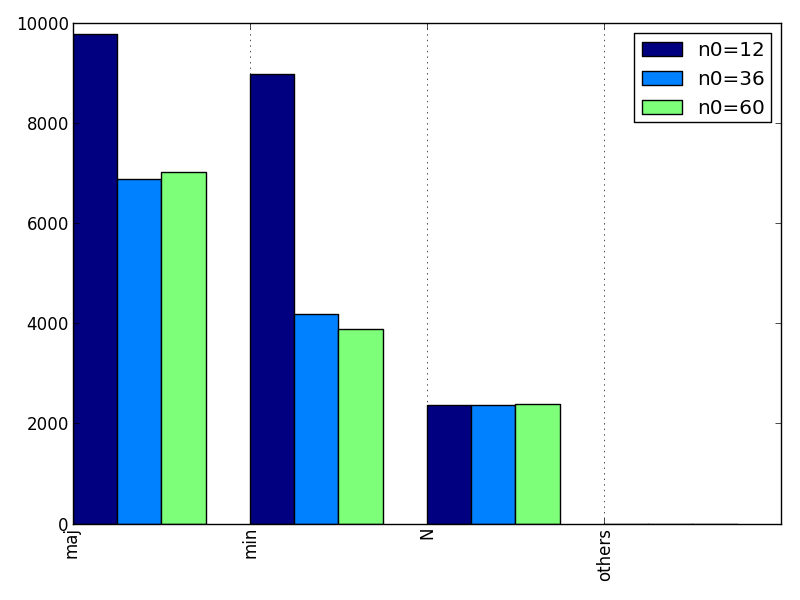
\includegraphics[scale=0.38]{errors/n03a} \\ а)}
  \end{minipage}
  \hfill
  \begin{minipage}[h]{0.49\linewidth}
    \center{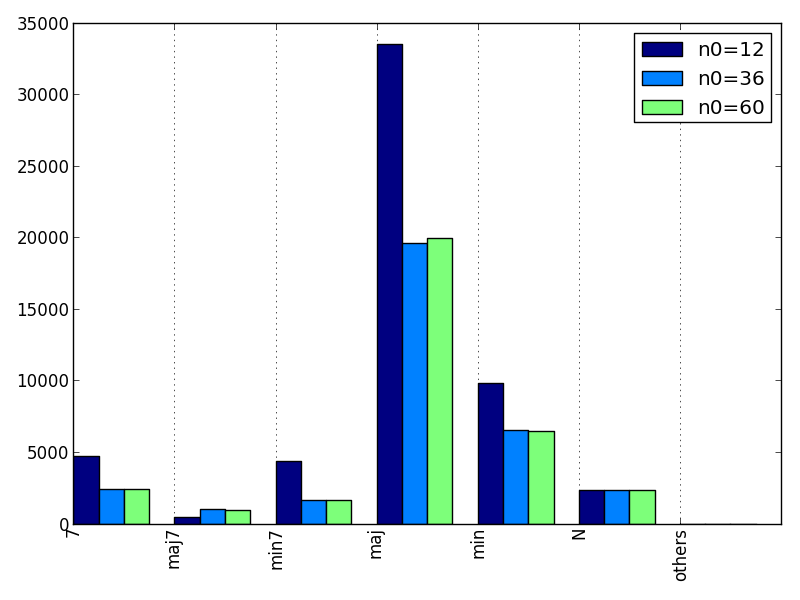
\includegraphics[scale=0.38]{errors/n04a} \\ б)}
  \end{minipage}
  \hfill
  \begin{minipage}[h]{0.49\linewidth}
    \center{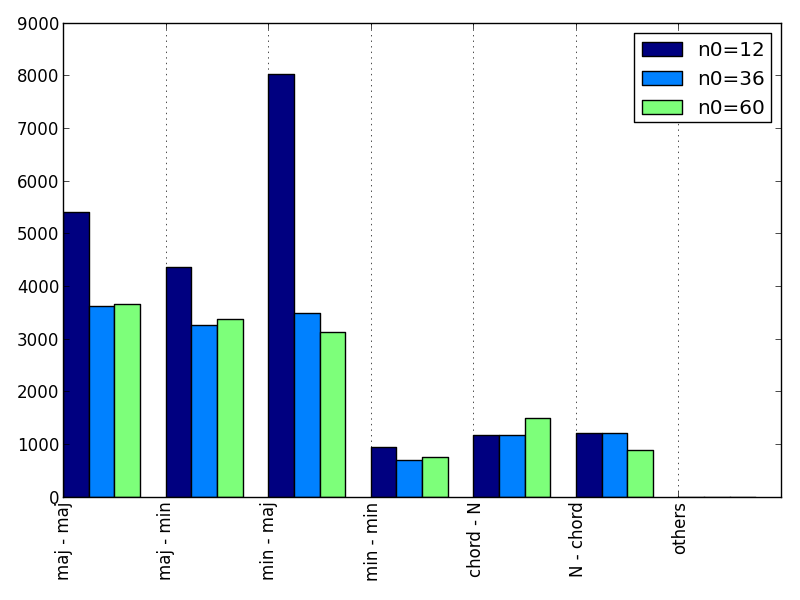
\includegraphics[scale=0.38]{errors/n03} \\ в)}
  \end{minipage}
  \hfill
  \begin{minipage}[h]{0.49\linewidth}
    \center{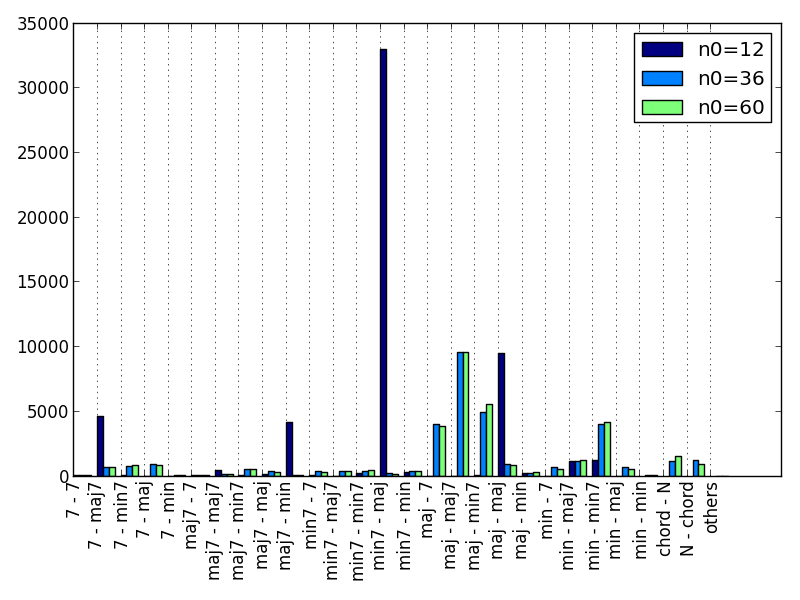
\includegraphics[scale=0.38]{errors/n04} \\ г)}
  \end{minipage}
  \caption{Диаграмма ошибок для разных значений $N_0$}
  \label{img:n0}
\end{figure}

В таблице \ref{TN0} приведены результаты, полученные при разных значениях
количества компонент преобразования постоянного качества, приходящихся на одну
октаву. Очевидно, что при наличии как минимум 36 компонент на октаву (3
компоненты на ноту) качество распознавания аккордов существенно повышается.
Различия между $N_0=36$ и $N_0=60$ не являются статистически значимыми. Однако
при $N_0=60$ требуется вычислить в 1.8 раз больше значений для компонент
преобразования постоянного качества, а также в дальнейшем многократно вычислять
дискретное косинусное преобразование для большего набора значений. Из рисунка
\ref{img:n0} видно, что значение $N_0=12$ не позволяет достаточно хорошо
различать мажорные и минорные аккорды. Огромное количество ошибок при таком
значении $N_0$ вызваны ошибочным 

\medskip

Эксперименты показывают безусловную важность реализованных методов для
улучшенного вычисления спектра. Повышение разрешения по времени с последующим
сглаживанием существенно повышает качество распознавания аккордов. Введение
задержки относительно моментов начала метрических долей также вносит свой вклад.
Использование более высокого разрешения по частоте при вычислении преобразования
постоянного качества позволяет использовать больше информации при сглаживании
спектрограммы. Преварительное определение ритма при помощи внешних библиотек и
предварительное определение частоты настройки при помощи реализованного
алгоритма улучшают качество полученной спектрограммы, позволяя вычислять
значения спектра для нужных частот в нужные моменты времени. Однако выбор
алгоритма определения ритма оказывает существенно более сильное влияние на
результат, чем выбор алгоритма определения частоты настройки.

% Основные вопросы относительно выбора параметров, возникающие на этом этапе:
% \begin{enumerate}
%   \item действительно ли определение частоты настройки музыкальных инструментов
%   повышает качество распознавания аккордов; (DONE)
%   \item каковы оптимальные параметры алгоритма определения частоты настройки;
%   \item действительно ли определение ритма повышает качество распознавания
%   аккордов; (DONE)
%   \item есть ли разница между библиотеками \emph{Beatroot} \cite{Dixon2007} и
%   \emph{Beat tracker} \cite{Davies2007} из набора \emph{Queen Mary Vamp
%   plugins}; (DONE)
%   \item возможно ли добиться при помощи быстрого преобразования Фурье и
%   последующего отображения полученного спектра на частоты звукоряда по формуле
%   \ref{fft_wrap} такого же качества распознавания, как при использовании
%   преобразования постоянного качества;
%   \item каковы оптимальные значения для разрешения по частоте $N_0$ (количество
%   компонент, приходящихся на октаву) и количества октав $N / N_0$ в
%   преобразовании постоянного качества; (DONE)
%   \item каковы оптимальные значения для количества вставляемых промежуточных
%   столбцов спектрограммы $T-1$ и размера окна при сглаживании $w$. (DONE)
% \end{enumerate}

% \begin{table} [htbp]
%   \centering
%   \parbox{15cm}{\caption{Название таблицы}\label{Ts0Sib}}
% %  \begin{center}
%   \begin{tabular}{| p{3cm} || p{3cm} | p{3cm} | p{4cm}l |}
%   \hline
%   \hline
%   Месяц   & \centering $T_{min}$, К & \centering $T_{max}$, К &\centering  $(T_{max} - T_{min})$, К & \\
%   \hline
%   Декабрь &\centering  253.575   &\centering  257.778    &\centering      4.203  &   \\
%   Январь  &\centering  262.431   &\centering  263.214    &\centering      0.783  &   \\
%   Февраль &\centering  261.184   &\centering  260.381    &\centering     $-$0.803  &   \\
%   \hline
%   \hline
%   \end{tabular}
% %  \end{center}
% \end{table}

\section{Преобразования спектрограммы} \label{sect3_specttrans}

На этом этапе необходимо оценить эффективность предложенных улучшений при
обработке спектрограммы: применение аналога фильтра Превитт, сглаживание с
использованием матрицы самоподобия. Также необходимо определить опитмальные
значения для количества зануляемых первых коэффициентов $\xi$ дискретного
косинусного преобразования, для доли сохраняемых в матрице самоподобия значений
$\zeta$.

\subsection{Применение аналога фильтра Превитт} \label{ssect3_prewitt}

В разделе \ref{sect1_feat} было предложено использовать аналог фильтра Превитт
для подавления компонент спектра, соответствующих шумовым звукам ударных
инструментов. Признаки CRP позволяют решить эту же задачу. Поэтому имеет смысл
сравнить итоговое качество распознавания аккордов с применением каждого из этих
методов в отдельности.

\begin{table} [htbp]
  \centering
  \parbox{15cm}{\caption{Влияние разных способов подавления шумовых звуков на
  качество распознавания аккордов} \label{TPrewitt}}
  \begin{tabular}{|l|l|l|l|}
  \hline
  Способ подавления & Triads & Tetrads & Сегментация \\
  \hline
  Превитт & 0.7492 & 0.5896 & 0.8063 \\
  Признаки CRP & 0.7720 & 0.4310 & 0.8141 \\
  Превитт + признаки CRP & 0.7524 & 0.5520 & 0.8066 \\
  \hline
  \end{tabular}
\end{table}

\begin{figure}[htbp]
  \begin{minipage}[h]{0.49\linewidth}
    \center{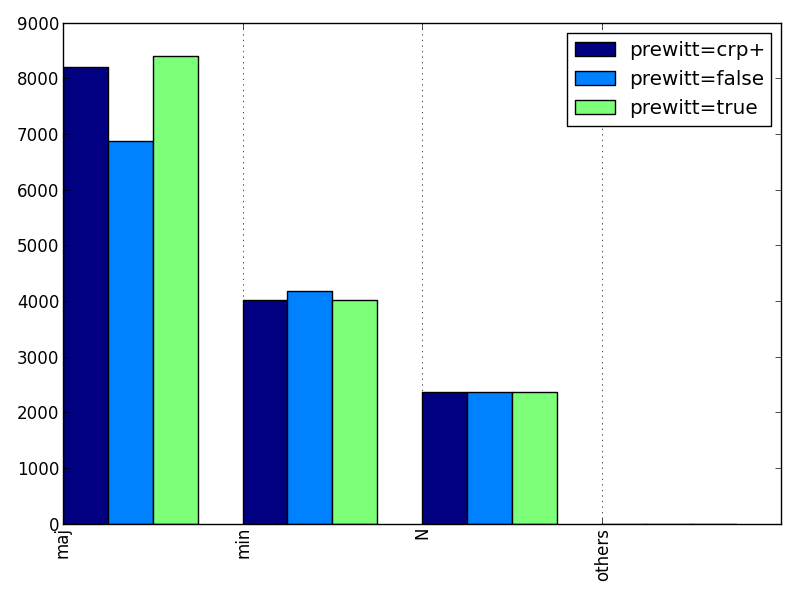
\includegraphics[scale=0.38]{errors/prewitt3a} \\ а)}
  \end{minipage}
  \hfill
  \begin{minipage}[h]{0.49\linewidth}
    \center{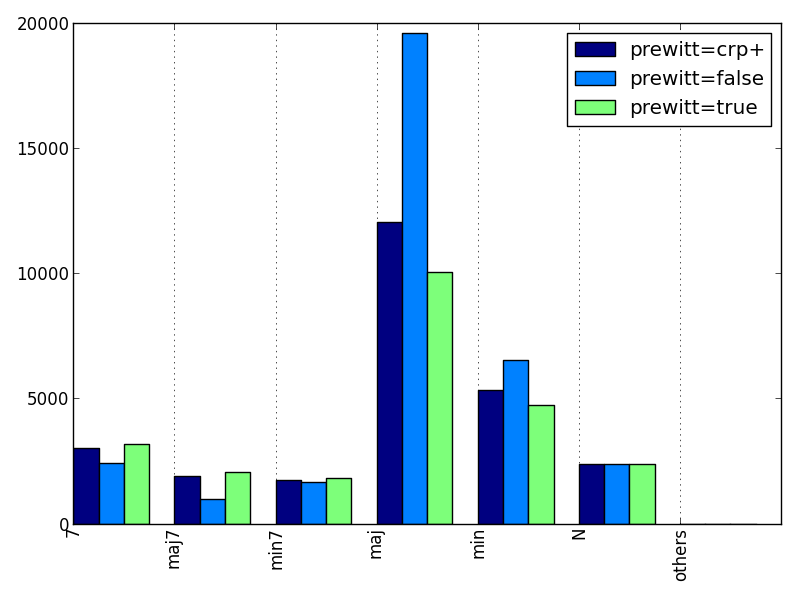
\includegraphics[scale=0.38]{errors/prewitt4a} \\ б)}
  \end{minipage}
  \caption{Диаграмма ошибок для разных способов подавления шумовых звуков}
  \label{img:prewitt}
\end{figure}

Результаты сравнения показаны в таблице \ref{TPrewitt}. К сожалению, применение
аналога фильтра Превитт только снижает качество распознавания аккордов,
независимо от того, будут ли далее применяться признаки CRP. Все попарные
различия между вариантами являются статистически значимыми.

\subsection{Настройка алгоритма вычисления признаков CRP} \label{ssect3_crp}

Вычисление признаков CRP включает в себя взятие логарифма от значений
спектрограммы, умноженных на коэффициент $\eta$. В работе \cite{Mueller2009},
описывающей этот тип признаков, предлагается выбирать $\eta$ из диапазона
100--10000. Далее к каждому столбцу спектрограммы применяется дискретное
косинусное преобразование. В полученном векторе зануляются первые $\xi$
значений, после чего к нему применяется обратное дискретное косинусное
преобразование. Необходимо определить влияние параметров $\eta$ и $\xi$ на
качество распознавания аккордов.

\begin{table} [htbp]
  \centering
  \parbox{15cm}{\caption{Влияние параметра $\eta$ на качество распознавания
  аккордов} \label{Teta}}
  \begin{tabular}{|l|l|l|l|}
  \hline
  $\eta$ & Triads & Tetrads & Сегментация \\
  \hline
  100 & 0.7348 & 0.4815 & 0.7971 \\
  1000 & 0.7652 & 0.5170 & 0.8102 \\
  10000 & 0.7721 & 0.4721 & 0.8139 \\
  50000 & 0.7720 & 0.4310 & 0.8141 \\
  100000 & 0.7719 & 0.4202 & 0.8144 \\
  \hline
  \end{tabular}
\end{table}

\begin{figure}[htbp]
  \begin{minipage}[h]{0.49\linewidth}
    \center{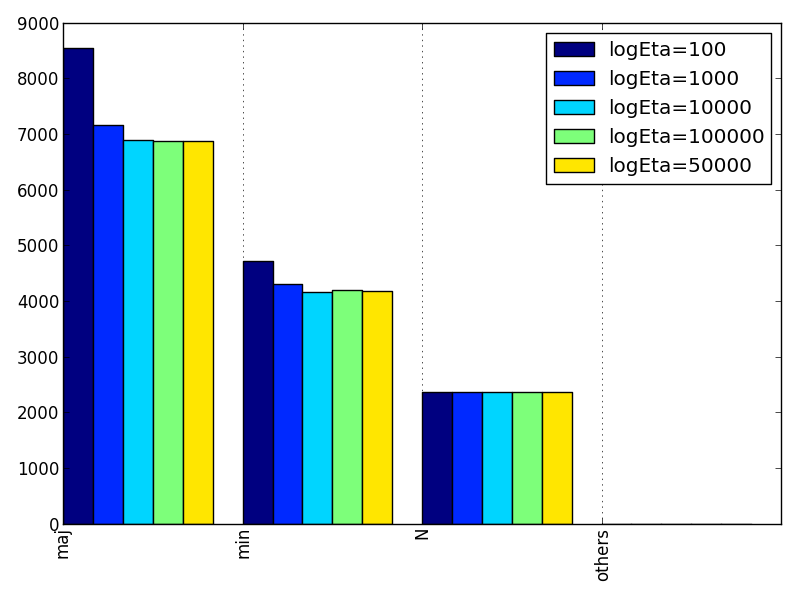
\includegraphics[scale=0.38]{errors/logEta3a} \\ а)}
  \end{minipage}
  \hfill
  \begin{minipage}[h]{0.49\linewidth}
    \center{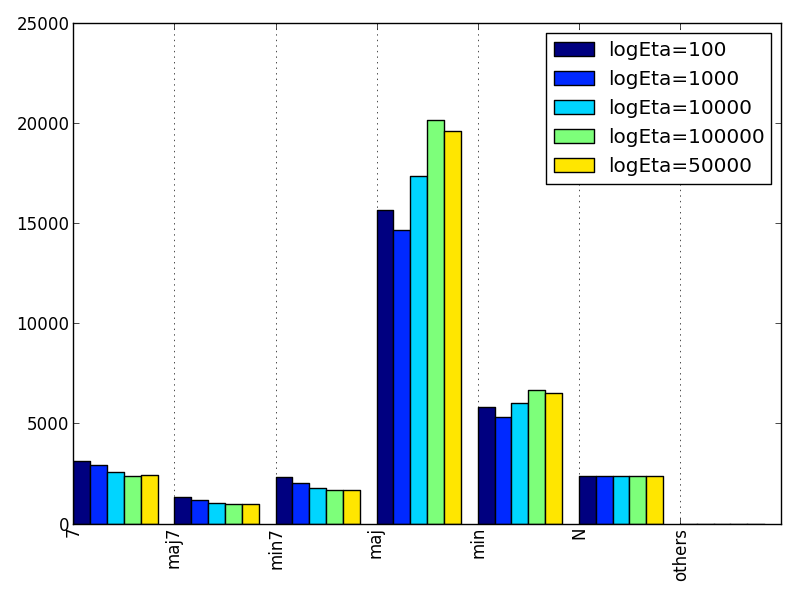
\includegraphics[scale=0.38]{errors/logEta4a} \\ б)}
  \end{minipage}
  \hfill
  \begin{minipage}[h]{0.49\linewidth}
    \center{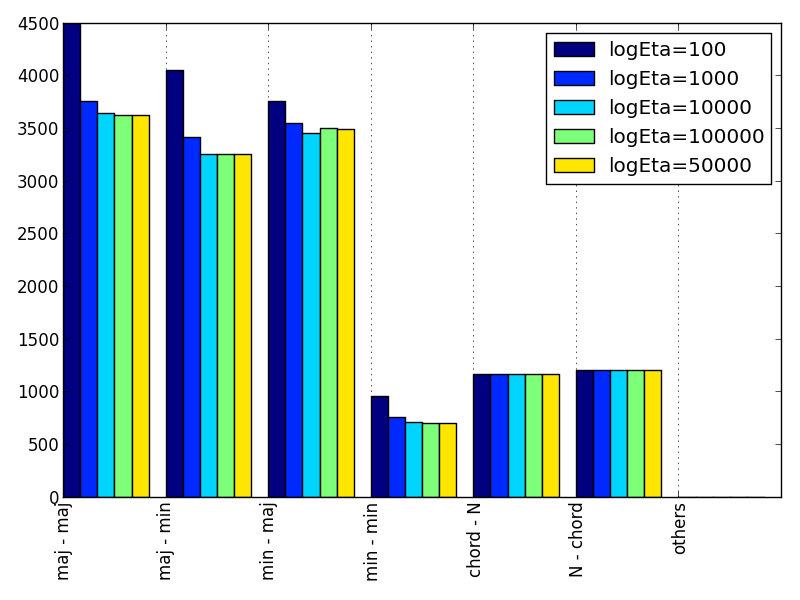
\includegraphics[scale=0.38]{errors/logEta3} \\ в)}
  \end{minipage}
  \hfill
  \begin{minipage}[h]{0.49\linewidth}
    \center{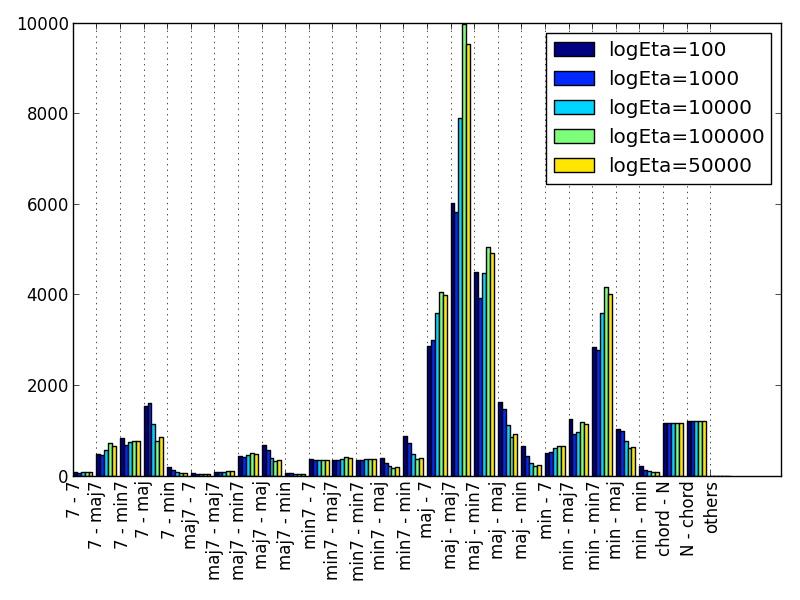
\includegraphics[scale=0.38]{errors/logEta4} \\ г)}
  \end{minipage}
  \caption{Диаграмма ошибок для разных значений $\eta$}
  \label{img:logEta}
\end{figure}

В \cite{Mueller2009} не было обнаружено существенных отличий между значениями
$\eta$ в диапазоне от 100 до 10000 применительно к задаче подавления тембра
музыкальных инструментов. Однако в задаче распознавания аккордов этот параметр
оказывает достаточно заметное влияние на результат. В таблице \ref{Teta}
показаны значения среднего перекрытия и сегментации для разных значений $\eta$
в промежутке от 100 до 100000. Наилучший результат для метрики ``Triads''
достигается при $\eta=10000$, $\eta=50000$, $\eta=100000$ (статистически
значимые различия отсутствуют). Все остальные различия являются статистически
значимыми.

При этом для метрики ``Tetrads'' наилучшие результаты получаются при меньших
значениях $\eta$. Из рисунка \ref{img:logEta} г) можно увидеть, что при больших
значениях $\eta$ растёт количество ошибочно определенных септаккордов вместо
соответствующих трезвучий.

Наилучшие результаты в \cite{Mueller2009} были получены для значений параметра
$\xi$ от 22 до 60 при 120-мерном векторе признаков. В этой работе в зависимости
от количества охватываемых октав и значения параметра $N_0$ размерность вектора
признаков (столбца спектрограммы) может меняться от 48 до 360. Значения в
таблице \ref{Txi} получены при охвате 4 октавы и $N_0=36$, что даёт 144-мерный
вектор признаков. Видно, что наилучшее качество распознавания аккордов
достигается при относительно небольших значениях $\xi$ с резким падением после
$\xi=20$. Только вариант $\xi=25$ статистически значимо отличается от всех
остальных. Из рисунков \ref{img:xi} в) и г) видно, что с увеличением $\xi$
растёт количество ошибочно определённых, соответственно, минорных трезвучий и
минорных септаккордов.

\begin{table} [htbp]
  \centering
  \parbox{15cm}{\caption{Влияние параметра $\xi$ на качество распознавания
  аккордов} \label{Txi}}
  \begin{tabular}{|l|l|l|l|}
  \hline
  $\xi$ & Triads & Tetrads & Сегментация \\
  \hline
  5 & 0.7671 & 0.3734 & 0.8067 \\
  10 & 0.773 & 0.4172 & 0.8138 \\
  15 & 0.7721 & 0.4310 & 0.8141 \\
  20 & 0.7705 & 0.3163 & 0.8128 \\
  25 & 0.7422 & 0.1667 & 0.8055 \\
  \hline
  \end{tabular}
\end{table}

\begin{figure}[htbp]
  \begin{minipage}[h]{0.49\linewidth}
    \center{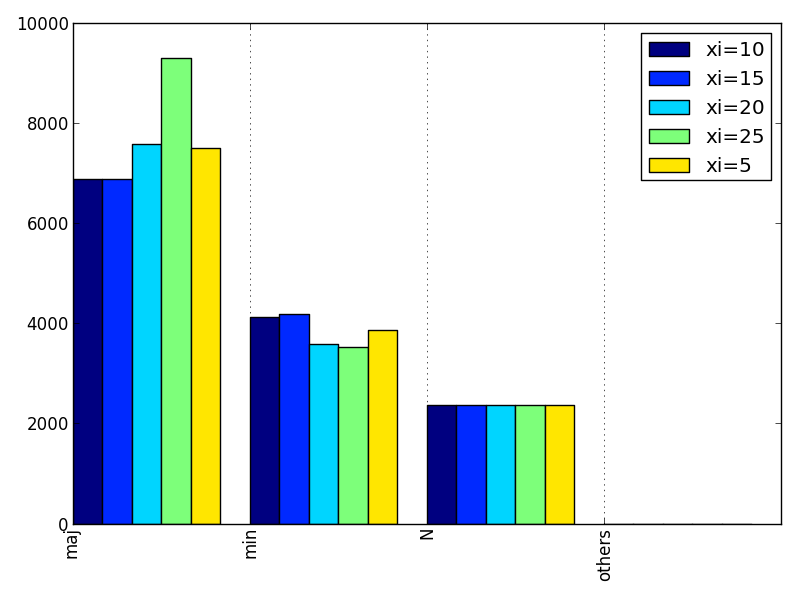
\includegraphics[scale=0.38]{errors/xi3a} \\ а)}
  \end{minipage}
  \hfill
  \begin{minipage}[h]{0.49\linewidth}
    \center{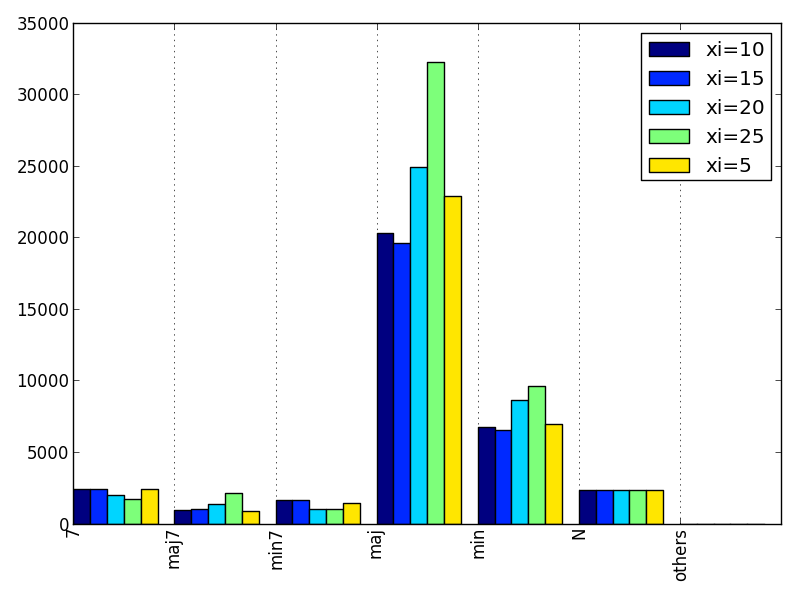
\includegraphics[scale=0.38]{errors/xi4a} \\ б)}
  \end{minipage}
  \hfill
  \begin{minipage}[h]{0.49\linewidth}
    \center{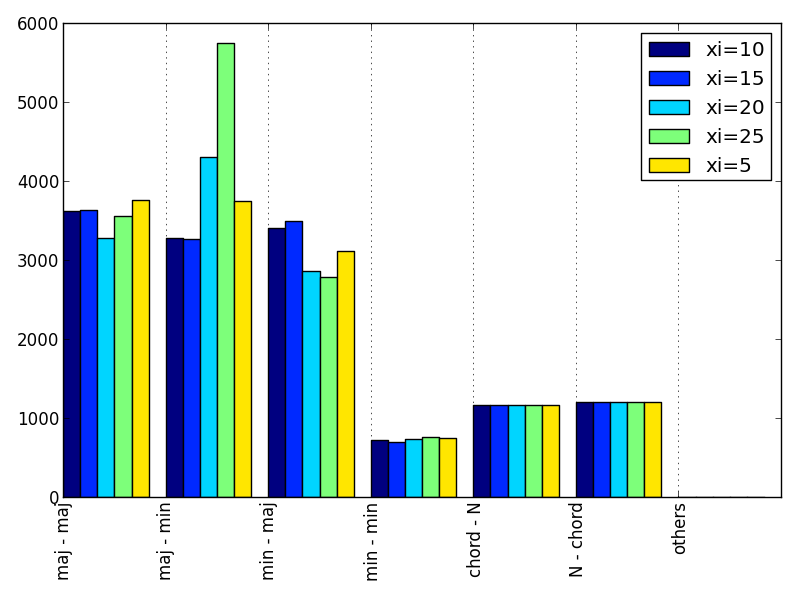
\includegraphics[scale=0.38]{errors/xi3} \\ в)}
  \end{minipage}
  \hfill
  \begin{minipage}[h]{0.49\linewidth}
    \center{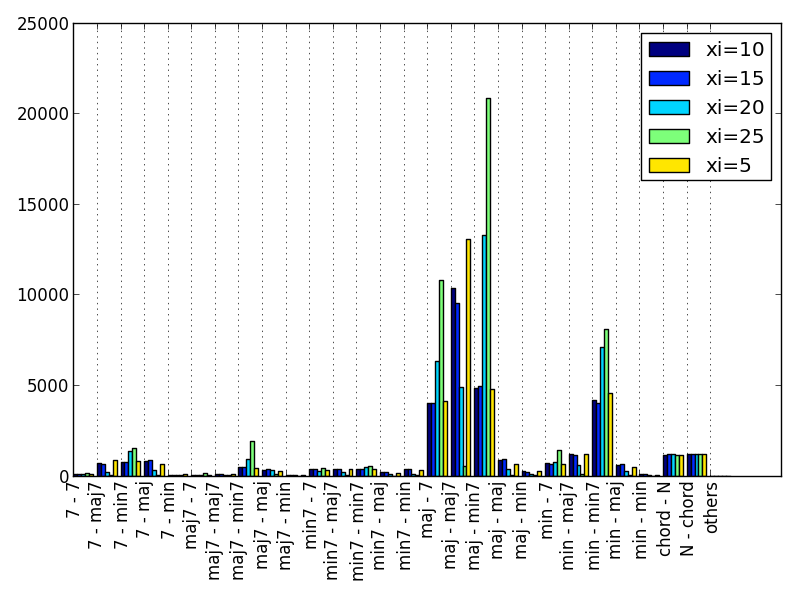
\includegraphics[scale=0.38]{errors/xi4} \\ г)}
  \end{minipage}
  \caption{Диаграмма ошибок для разных значений $\xi$}
  \label{img:xi}
\end{figure}

\subsection{Применение самоподобия} \label{ssect3_selfsim}

При использовании матрицы самоподобия для улучшения спектрограммы необходимо
выбрать наилушее значение для параметра $\zeta$. Этот параметр контролирует
долю столбцов спектрограммы, наиболее схожих с тем, который корректируется в
данный момент.

\begin{table} [htbp]
  \centering
  \parbox{15cm}{\caption{Влияние параметра $\zeta$ на качество распознавания
  аккордов} \label{Tzeta}}
  \begin{tabular}{|l|l|l|l|}
  \hline
  $\zeta$ & Triads & Tetrads & Сегментация \\
  \hline
  0 & 0.7001 & 0.5535 & 0.7827 \\
  0.05 & 0.7716 & 0.4204 & 0.8147 \\
  0.1 & 0.7720 & 0.4310 & 0.8141 \\
  0.15 & 0.7663 & 0.4313 & 0.8086 \\
  \hline
  \end{tabular}
\end{table}

\begin{figure}[htbp]
  \begin{minipage}[h]{0.49\linewidth}
    \center{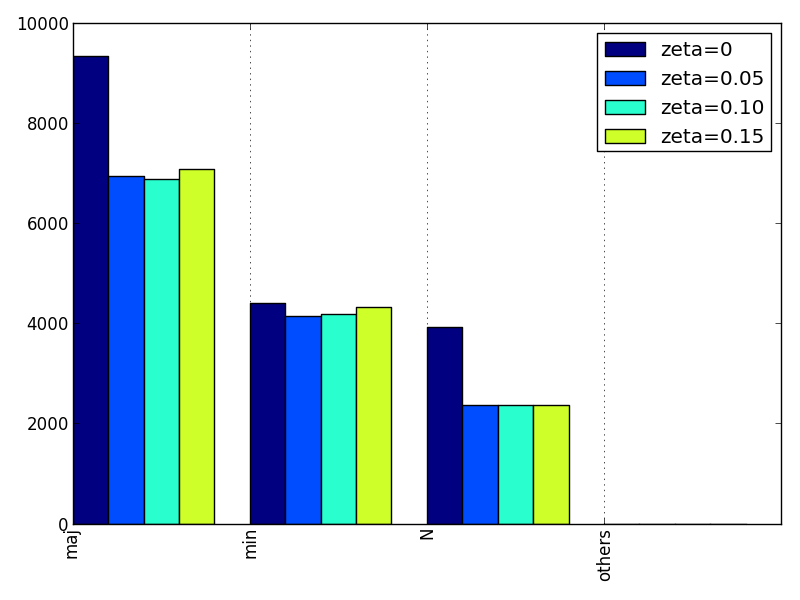
\includegraphics[scale=0.38]{errors/zeta3a} \\ а)}
  \end{minipage}
  \hfill
  \begin{minipage}[h]{0.49\linewidth}
    \center{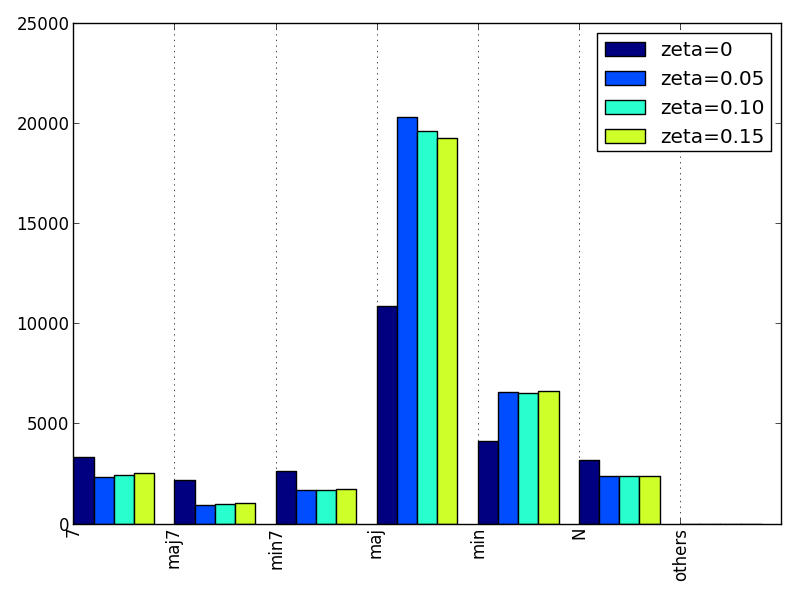
\includegraphics[scale=0.38]{errors/zeta4a} \\ б)}
  \end{minipage}
  \caption{Диаграмма ошибок для разных значений $\zeta$}
  \label{img:zeta}
\end{figure}

В таблице \ref{Tzeta} приведены значения среднего перекрытия и сегментации для
разных значений $\zeta$. Различия между наилучшими вариантами $\zeta=0.05$,
$\zeta=0.1$ и $\zeta=0.15$ не являются статистически значимыми. Значение
$\zeta=0$ соответствует отсутствию коррекции спектрограммы при помощи
самоподобия. Полученные при этом значении $\zeta$ результаты оказываются
существенно хуже, чем при ненулевых значениях $\zeta$.

В работах \cite{Mauch2010} и \cite{Cho2011} отмечалось положительное влияние от
коррекции последовательности векторов признаков с использованием наиболее
близких друг к другу векторов. Однако в обеих указанных работах строились
матрицы самоподобия для 12-мерных хроматических векторов, в то время как в
таблице \ref{Tzeta} все значения получены с использованием матрицы самоподобия
для столбцов спектрограммы. После применения аналогичного метода к хроматическим
векторам при $\zeta=0.08$ были получены значения для взвешенного среднего
перекрытия и сегментации, соответственно, $0.7620$ и $0.8119$. Результат
оказался статистически значимо хуже (в соответствии с критерием Вилкоксона).

\medskip

Использование признаков CRP позволяет более эффективно подавлять шумовые
компоненты в спектре по сравнению с применением аналога фильтра Превитт. Эти
признаки были предложены в \cite{Mueller2009} для решения другой задачи, поэтому
другими были и оптимальные диапазоны для параметров этих признаков. Коррекция
спектрограммы с использованием очищенной матрицы самоподобия приводит к очень
существенному повышению качества распознавания аккордов и, таким образом,
является одним из самых важных шагов в реализованном алгоритме.

% Основные вопросы относительно выбора параметров, возникающие на этом этапе:
% \begin{enumerate}
%   \item действительно ли применение аналога фильтра Превитт повышает качество
%   распознавания акокрдов; (DONE)
%   \item каково оптимальное значение для количества зануляемых первых
%   коэффициентов дискретного косинусного преобразования $\xi$ при вычислении
%   признаков CRP; (DONE)
%   \item действительно ли сглаживание с использованием матрицы самоподобия для
%   столбцов спектрограммы лучше, чем с использованием такой матрицы для векторов
%   признаков и без использования самоподобия вообще; (DONE)
%   \item каково оптимальное значение для доли сохраняемых в матрице самоподобия
%   значений $\zeta$. (DONE)
% \end{enumerate}

\section{Нейронные сети} \label{sect3_nn}

Для нейронной сети необходимо определить оптимальные значения для
метапараметров, которые задаются изначально и не изменяются в процессе обучения.
Это, прежде всего, конфигурация сети: количество скрытых слоёв и количество
нейронов во входном и в скрытых слоях, наличие рекуррентных соединений.

Нейронная сеть была реализована на языке \emph{Python} с использованием пакета
\emph{Theano} \cite{Bergstra2010}. Обучающие данные делились на мини-пакеты по 5
векторов в каждом. Предварительное обучение каждого слоя с помощью
автоассоциатора производилось в течение 15 эпох. Окончательное обучение
нейронной сети также продолжалось в течение 15 эпох.

Рекуррентные соединения добавлялись к последнему из слоёв, обучаемых при помощи
автоассоциаторов. При окончательном обучении рекуррентных вариантов сети
сохранялась исходная последовательность обучающих векторов. При предварительном
обучении слоёв и при окончательном обучении нерекуррентных вариантов обучающие
векторы перемешивались в случайном порядке.

Для проведения экспериментов тестовая коллекция из 318 композиций была случайным
образом поделена на 2 равные части, каждая из которых поочередно выступала в
качестве обучающей и тестовой выборки.

В экспериментах предварительно вычисленные спектрограммы звукозаписей по
столбцам подавались на вход нейронной сети. Описанные в параграфах
\ref{sect1_feat} и \ref{sect1_selfsim} преобразования к спектрограмме не
применялись, за исключением взятия логарифма от её компонент. Однако матрица
самоподобия использовалась для сглаживания последовательности хроматических
векторов, полученных на выходе нейронной сети. При определении
последовательности аккордов использовались эвристики, описанные в параграфе
\ref{sect1_class}.

\subsection{Конфигурация нейронной сети}

Были рассмотрены различные варианты нерекуррентных сетей (SDA) с 48 и с 60
входами (охватывающие, соответственно, 4 или 5 октав звукозаписи), имеющие 1, 2
или 3 скрытых слоя с разными количествами нейронов. Для всех сетей были
рассмотрены также соответствующие рекуррентные варианты (RSDA). Соответствующие
результаты приведены в таблице \ref{Tnnconf}. В названии конфигурации первое
число в скобках соответствует количеству входов, остальные -- количеству
нейронов в скрытых слоях.

\begin{table} [htbp]
  \centering
  \parbox{15cm}{\caption{Влияние конфигурации нейронной сети на качество
  распознавания аккордов} \label{Tnnconf}}
  \begin{tabular}{|l|l|l|l|}
  \hline
  Конфигурация & Triads & Tetrads & Сегментация \\
  \hline
  SDA (48, 200) & 0.7639 & 0.6234 & 0.8035 \\
  SDA (48, 200, 200) & 0.7616 & 0.6316 & 0.8009 \\
  SDA (60, 100) & 0.7616 & 0.6279 & 0.7991 \\
  SDA (60, 200) & 0.7637 & 0.6314 & 0.8010 \\
  SDA (60, 300) & 0.7649 & 0.6322 & 0.8011 \\
  SDA (60, 200, 100) & 0.7664 & 0.6389 & 0.8011 \\
  SDA (60, 300, 300) & 0.7650 & 0.6363 & 0.8012 \\
  SDA (60, 100, 100, 100) & 0.7671 & 0.6382 & 0.7996 \\
  SDA (60, 300, 300, 300) & 0.7674 & 0.6373 & 0.8011 \\
  \hline
  RSDA (48, 200) & 0.7616 & 0.6226 & 0.7963 \\
  RSDA (48, 200, 200) & 0.7660 & 0.6342 & 0.7982 \\
  RSDA (60, 300) & 0.7613 & 0.6298 & 0.7955 \\
  RSDA (60, 300, 300) & 0.7672 & 0.6373 & 0.7982 \\
  RSDA (60, 300, 300, 300) & 0.7686 & 0.6360 & 0.7986 \\
  \hline
  \end{tabular}
\end{table}

Несмотря на то, что конфигурации с большим количеством нейронов показали чуть
более высокие результаты, по итогам экспериментов не выявлено существенных
различий в качестве распознавания аккордов между разными конфигурациями
нейронной сети. Полученные результаты достаточно близки, и лишь в нескольких
парах есть статистически значимые различия. При этом обучение нейронных сетей с
рекуррентым слоем и последующее их тестирование отнимает значительно больше
времени, чем для сетей без рекуррентного слоя (см. раздел \ref{sect3_time}).
Количество нейронов во входном слое несущественно влияет на время работы, но
большее их количество приводит к чуть лучшему результату. С учётом высказанных
соображений, в дальнейших экспериментах было решено использовать конфигурацию
SDA (60, 300, 300).

\subsection{Влияние логарифмирования спектрограммы}

Как видно из таблицы \ref{Tnnlog}, применение логарифмического преобразования к
столбцам спектрограммы при обучении нейронной сети и при последующем её
использовании позволяет существенно улучшить качество распознавания аккордов.

\begin{table} [htbp]
  \centering
  \parbox{15cm}{\caption{Влияние логарифмирования спектрограммы до применения
  нейронной сети на качество распознавания аккордов} \label{Tnnlog}}
  \begin{tabular}{|l|l|l|l|}
  \hline
  Конфигурация & Triads & Tetrads & Сегментация \\
  \hline
  SDA (60, 300, 300) nolog & 0.7350 & 0.6050 & 0.7890 \\
  SDA (60, 300, 300) & 0.7672 & 0.6373 & 0.7982 \\
  \hline
  \end{tabular}
\end{table}

Таким образом, предварительная обработка данных имеет смысл также и при
использовании нейронной сети для получения признаков на их основе.

\subsection{Влияние зашумления на этапе предварительного обучения}
\label{ssect3_noise}

Как описано в разделе \ref{sect2_sda}, при предварительном обучении слоёв
нейронной сети входные векторы зашумляются. В таблица \ref{Tnnnoise} приведены
результаты, полученные для конфигурации SDA (60, 300, 300) при различных типах
шума и разных значениях параметра, контролирующего уровень шума: дисперсия для
аддитивного шума ($0$ соответствует его отсутствию), вероятность обнуления
компоненты входного вектора -- для маскирующего шума.

\begin{table} [htbp]
  \centering
  \parbox{15cm}{\caption{Влияние зашумления на этапе предварительного обучения
  нейронной сети на качество распознавания аккордов} \label{Tnnnoise}}
  \begin{tabular}{|l|l|l|l|l|}
  \hline
  Параметр & Тип шума & Triads & Tetrads & Сегментация \\
  \hline
  0.2 & аддитивный & 0.7668 & 0.6361 & 0.8013 \\
  \hline
  0.2 & маскирующий & 0.7677 & 0.6336 & 0.8018 \\
  \hline
  \end{tabular}
\end{table}

Ни один из вариантов зашумления (включая его отсутствие) не приводит к
результату, статистически значимо отличающемуся от всех остальных.

\subsection{Влияние циклических сдвигов на этапе тестирования}
\label{ssect3_cycletest}

Циклический сдвиг для векторов признаков или входных данных часто применяется на
этапе обучения модели, но обычно не применяется при тестировании (зачастую,
например, при использовании СММ, это излишне усложняет алгоритм). Предложенный в
параграфе \ref{sect2_sda} метод для использования циклического сдвига на этапе
тестирования модели не приводит к заметному усложнению этого этапа. Увеличение
количества вычислений в 12 раз не очень заметно, учитывая относительно небольшое
время обработки спектра нейронной сетью в процессе тестирования.

\begin{table} [htbp]
  \centering
  \parbox{15cm}{\caption{Влияние циклических сдвигов на этапе тестирования
  нейронной сети на качество распознавания аккордов}
  \label{Tnncyctest}}
  \begin{tabular}{|l|l|l|l|}
  \hline
  Конфигурация & Triads & Tetrads & Сегментация \\
  \hline
  SDA (60, 300, 300) nocycle & 0.7703 & 0.6261 & 0.8020 \\
  SDA (60, 300, 300) & 0.7672 & 0.6373 & 0.7982 \\
  \hline
  \end{tabular}
\end{table}

Как видно из таблицы \ref{Tnncyctest}, помимо некоторого увеличения времени
обработки, это приводит даже к небольшому ухудшению результата (в метрике
<<Triads>>). Вероятно, применение циклических сдвигов на этапе обучения
нейронной сети является достаточным, и дополнительные действия на этапе
тестирования не требуются.

\medskip

Хроматические векторы, полученные с использованием многослойных нейронных сетей,
позволяют получить сравнимые с традиционными хроматическими признаками
результаты распознавания аккордов. Вместе с тем, качество полученных
хроматических векторв зависит от предварительной обработки спектральных данных
гораздо больше, чем от конфигурации самой нейронной сети и метода зашумления
исходных данных при предварительном обучении. Добавление нейронов, слоёв и
рекуррентных соединений влияет на продолжительность обучения модели в гораздо
большей степени, чем на итоговое качество распознавания аккордов.

\section{Классификация векторов признаков} \label{sect3_class}

Для определения последовательности аккордов по полученной последовательности
хроматических векторов используется простой метод ближайшего соседа. Для этого
строятся шаблонные хроматческие векторы для всех аккордов из множества
распознаваемых аккордов $Y$. При построении шаблонов используются 2 параметра:
количество учитываемых обертонов и вклад $h$ этих обертонов в шаблон (в
соответствии с формулой (\ref{eq:templates_harmonics})). Затем для каждого
вектора из последовательности определяются расстояния от него до всех шаблонных
векторов. Необходимо рассмотреть разные способы определения расстояния.

\subsection{Шаблонные векторы} \label{ssect3_templates}

Поскольку первый обертон любой ступени звукоряда соответствует звуку с таким же
названием, нет смысла рассматривать отдельно случай шаблонов без обертонов. Но,
учитывая экспоненциальный характер убывания вклада каждого последующего обертона
в шаблоны, имеет смысл рассматривать достаточно небольшое их количество. В
\cite{Oudre2009} авторы ограничиваются первыми пятью обертонами. В соответствии
с формулой (\ref{eq:templates_harmonics})) при $h=0.6$ вклад пятого обертона
будет составлять $0.6^5 \approx 0.078$ от вклада первого, то есть более чем в 12
раз слабее. Поэтому вряд ли имеет смысл рассматривать большее их количество.

\begin{table} [htbp]
  \centering
  \parbox{15cm}{\caption{Влияние количества обертонов в шаблонах на качество
  распознавания аккордов} \label{Tover}}
  \begin{tabular}{|l|l|l|l|}
  \hline
  Количество обертонов & Triads & Tetrads & Сегментация \\
  \hline
  1 & 0.7516 & 0.1586 & 0.8064 \\
  2 & 0.7720 & 0.4310 & 0.8141 \\
  3 & 0.7706 & 0.3611 & 0.8139 \\
  4 & 0.7680 & 0.5713 & 0.8134 \\
  5 & 0.7703 & 0.6173 & 0.8137 \\
  \hline
  \end{tabular}
\end{table}

\begin{figure}[htbp]
  \begin{minipage}[h]{0.49\linewidth}
    \center{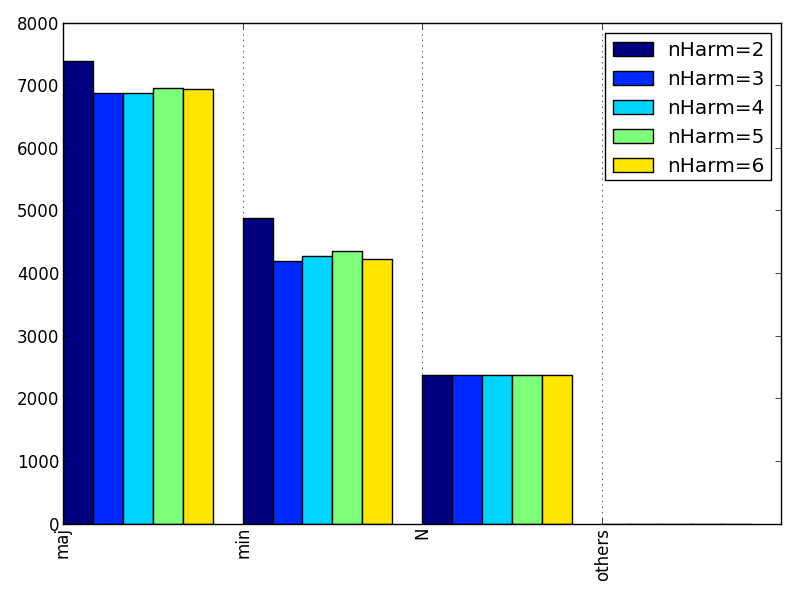
\includegraphics[scale=0.38]{errors/nHarm3a} \\ а)}
  \end{minipage}
  \hfill
  \begin{minipage}[h]{0.49\linewidth}
    \center{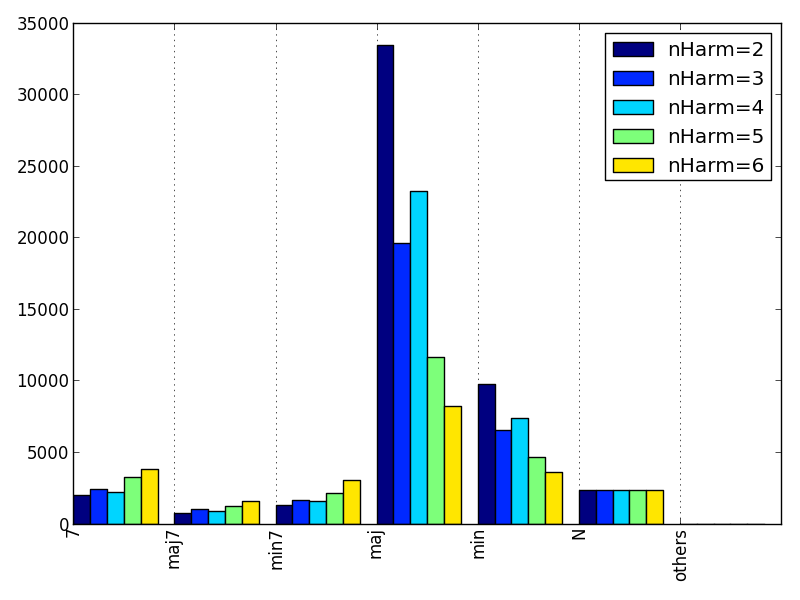
\includegraphics[scale=0.38]{errors/nHarm4a} \\ б)}
  \end{minipage}
  \caption{Диаграмма ошибок при разных количествах обертонов в шаблонах}
  \label{img:nHarm}
\end{figure}

В таблице \ref{Tover} показаны результаты экспериментов в зависимости от
количества учитываемых в шаблонах обертонов. Различия между 2 и 3 обертонами, а
также между 3, 4 и 5 обертонами, не являются статистически значимыми, но
максимум наблюдается при использовании в шаблонах 2 обертонов дополнительно к
основному тону.

Коэффициент $h$ убывания вклада обертонов в \cite{Gomez2006} и \cite{Oudre2009}
выбирается равным 0.6, его влияние в этих работах не исследуется. В таблице
\ref{Th} приведены значения взвешенного среднего перекрытия и сегментации,
полученные автором для разных значений $h$. Для случаев $h=0.5$, $h=0.6$,
$h=0.7$ статистически значимые различия не обнаружены, но их отличия от
вариантов $h=0.4$, $h=0.8$ являются статистически значимыми. В целом, влияние
данного параметра достаточно слабое.

\begin{table} [htbp]
  \centering
  \parbox{15cm}{\caption{Влияние коэффициента убывания вклада обертона на
  качество распознавания аккордов} \label{Th}}
  \begin{tabular}{|l|l|l|l|}
  \hline
  $h$ & Triads & Tetrads & Сегментация \\
  \hline
  0.4 & 0.7660 & 0.2038 & 0.8121 \\
  0.5 & 0.7694 & 0.2881 & 0.8135 \\
  0.6 & 0.7720 & 0.4310 & 0.8141 \\
  0.7 & 0.7733 & 0.5749 & 0.8133 \\
  0.8 & 0.7708 & 0.6216 & 0.8114 \\
  \hline
  \end{tabular}
\end{table}

\begin{figure}[htbp]
  \begin{minipage}[h]{0.49\linewidth}
    \center{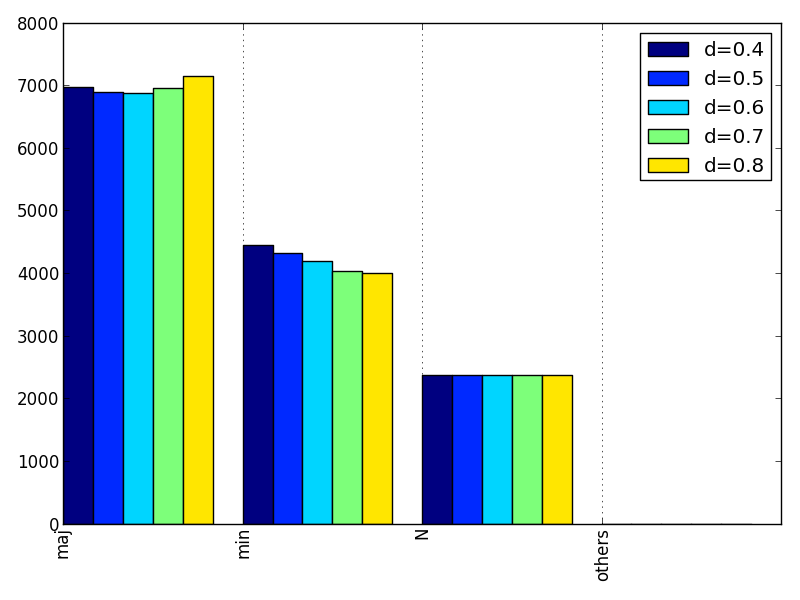
\includegraphics[scale=0.38]{errors/d3a} \\ а)}
  \end{minipage}
  \hfill
  \begin{minipage}[h]{0.49\linewidth}
    \center{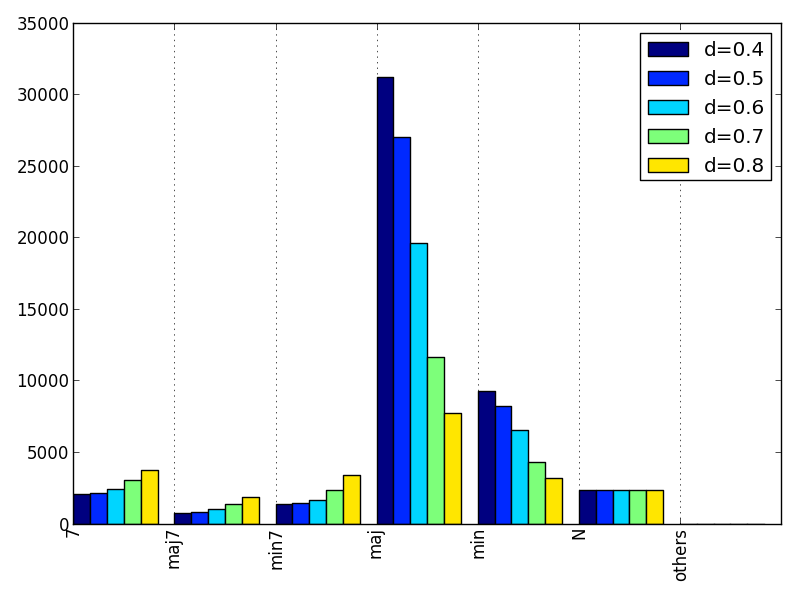
\includegraphics[scale=0.38]{errors/d4a} \\ б)}
  \end{minipage}
  \caption{Диаграмма ошибок для разных значений $h$}
  \label{img:h}
\end{figure}

Примечательно (см. рисунки \ref{img:h}, \ref{img:nHarm}), что параметры шаблонов
не оказывают почти никакого влияния в случае распознавания только мажорных и
минорных трезвучий, но сильно влияют на результат при распознавании
септаккордов. Это можно объяснить тем, что получаемые в реальности 12-мерные
тональные векторы не являются бинарными. Определённое количество звуковой
энергии приходится на все их компоненты. А поскольку шаблоны для септаккордов
учитывают гармоники 4 тональных классов, почти все их компоненты оказываются
ненулевыми. За счёт этого расстояние от таких шаблонов до полученных тональных
векторов оказывается меньше, и септаккорд определяется там, где на самом деле
звучит мажорное или минорное трезвучие. Для частичной компенсации этого эффекта
количество гармоник в шаблонах для септаккордов было ограничено двумя. С
увеличением же количества гармоник и вклада каждой из последующих гармоник
энергия в шаблонах для трезвучий распределяется более равномерно. В результате
эти шаблоны оказываются более подходящими для отделения трезвучий от
септаккордов.

\begin{figure}[htbp]
  \begin{minipage}[h]{0.49\linewidth}
    \center{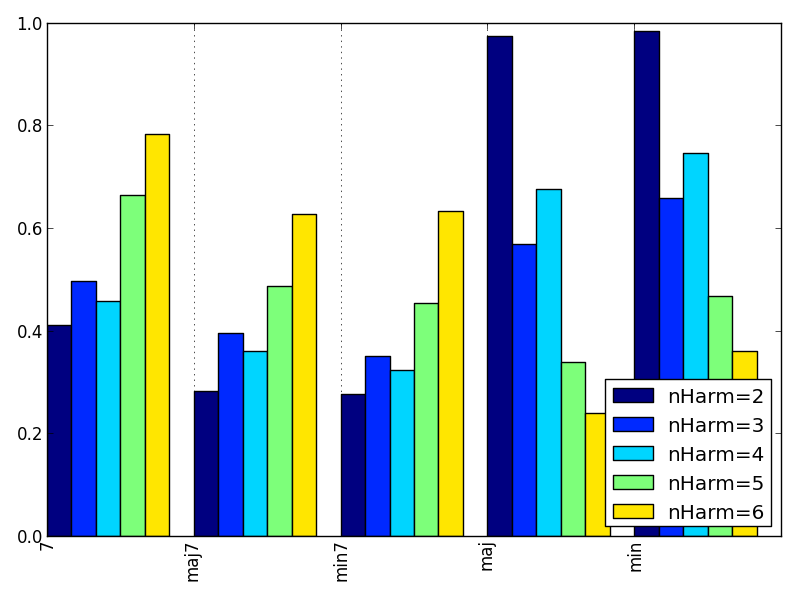
\includegraphics[scale=0.38]{errors/nHarm4n} \\ а)}
  \end{minipage}
  \hfill
  \begin{minipage}[h]{0.49\linewidth}
    \center{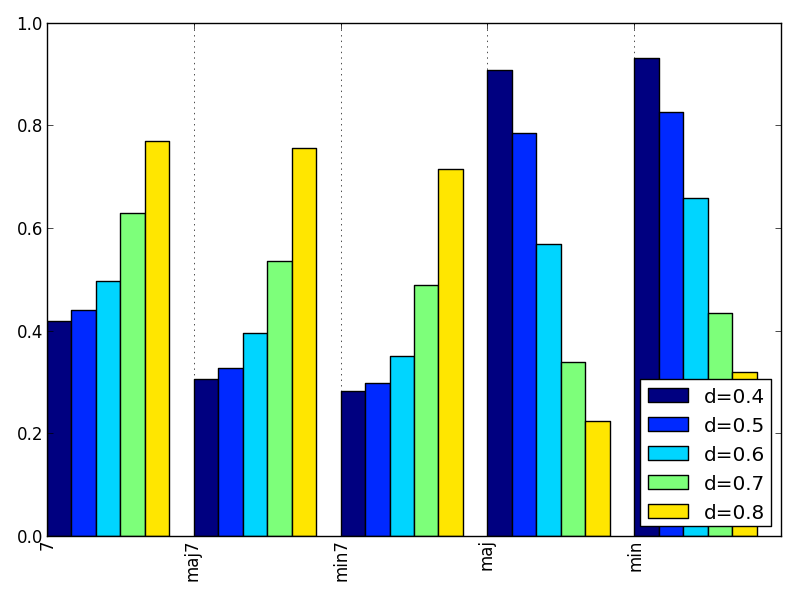
\includegraphics[scale=0.38]{errors/d4n} \\ б)}
  \end{minipage}
  \caption{Нормализованная диаграмма ошибок для разных значений количества
  обертонов и параметра $h$}
  \label{img:nHarmh_n}
\end{figure}

Вспомним, что в совокупности все фрагменты, на которых звучат септаккорды,
составляют лишь чуть более 20\% от длительности тестовой коллекции (см. таблицу
\ref{Tchord_stat}). Поэтому падение количества ошибок на септаккордах может
оказаться менее важным, чем рост количества ошибок на мажорных и минорных
трезвучиях. На рисунке \ref{img:nHarmh_n} высота столбцов соответствует доле
фрагментов с аккордами каждого из типов, на которых была сделана ошибка
распознавания. Видно, что в действительности уменьшение количества ошибок
распознавания трезвучий компенсируется ростом количества ошибок распознавания
септаккордов. Но из-за существенно меньшей доли фрагментов с септаккордами в
коллекции значение метрики ``Tetrads'' растёт. Нельзя говорить, однако, что при
больших значениях параметра $h$ или количества гармоник в шаблонах алгоритм
лучше распознаёт септаккорды.

\subsection{Эвристики} \label{ssect3_heuristics}

\begin{table} [htbp]
  \centering
  \parbox{15cm}{\caption{Влияние эвристик на качество распознавания аккордов}
  \label{THeuristics}}
  \begin{tabular}{|l|l|l|l|}
  \hline
  Эвристики & Triads & Tetrads & Сегментация \\
  \hline
  Без эвристик & 0.7634 & 0.4341 & 0.8083 \\
  Исправление одиночных аккордов & 0.7721 & 0.4393 & 0.8164 \\
  Исправление типа аккорда & 0.7655 & 0.4270 & 0.8141 \\
  Обе эвристики & 0.7720 & 0.4310 & 0.8141 \\
  \hline
  \end{tabular}
\end{table}

Изменения результата при использовании предложенных эвристик показаны в таблице
\ref{THeuristics}. Как видно, исправление типа аккорда оказывается, фактически,
бесполезным. Однако исправление аккордов, которые продолжаются в течение только
одной метрической доли, имеет заметный эффект и даёт статистически значимое
улучшение качества распознавания аккордов.

\subsection{Определение отсутствия аккорда} \label{ssect3_noChord}

Параметр $L_N$, описанный в параграфе \ref{ssect1_noChord}, позволяет
определить, для каких столбцов спектрограммы будет определяться отсутствие
звучащего аккорда. В таблице \ref{TLN} приведены результаты экспериментов для
разных значений $L_N$. При $L_N \leq 0.0025$ результат изменяться перестаёт, то
есть, фактически, все столбцы спектрограммы считаются содержащими аккорд. При
значениях $L_N > 0.003$ результат существенно падает, поскольку, наоборот,
появляется слишком много столбцов, для которых определяется отсутствие аккорда.
Это можно заметить на рисунке \ref{img:noChordness}. Наилучший результат был
получен при $L_N = 0.003$, но статистически значимых отличий между ним и
результатами при меньших значениях $L_N$ нет.

\begin{table} [htbp]
  \centering
  \parbox{15cm}{\caption{Влияние порога для отсутствия аккорда на
  качество распознавания аккордов} \label{TLN}}
  \begin{tabular}{|l|l|l|l|}
  \hline
  $L_N$ & Triads & Tetrads & Сегментация \\
  \hline
  0.0015 & 0.7720 & 0.4310 & 0.8141 \\
  0.0020 & 0.7720 & 0.4310 & 0.8141 \\
  0.0025 & 0.7724 & 0.4314 & 0.8141 \\
  0.0030 & 0.7756 & 0.4365 & 0.8140 \\
  0.0035 & 0.7075 & 0.4279 & 0.7720 \\
  \hline
  \end{tabular}
\end{table}

\begin{figure}[htbp]
  \begin{minipage}[h]{0.49\linewidth}
    \center{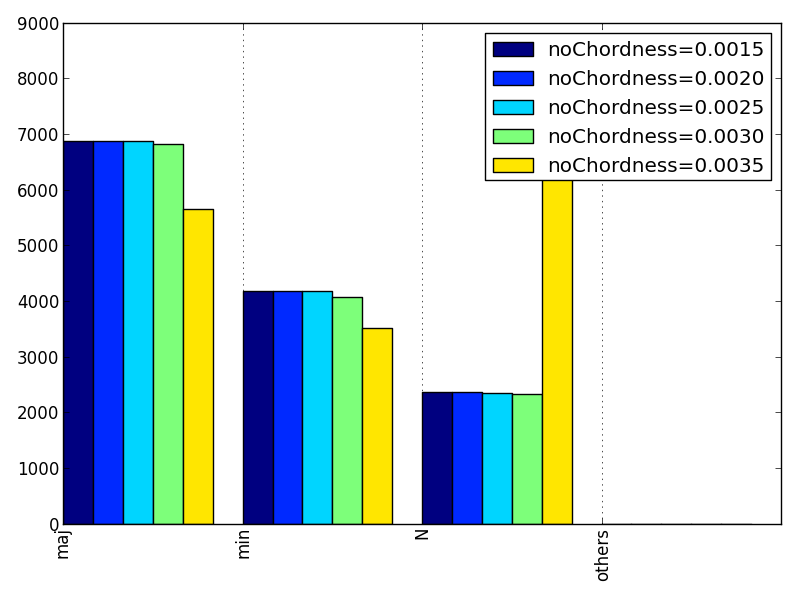
\includegraphics[scale=0.38]{errors/noChordness3a} \\ а)}
  \end{minipage}
  \hfill
  \begin{minipage}[h]{0.49\linewidth}
    \center{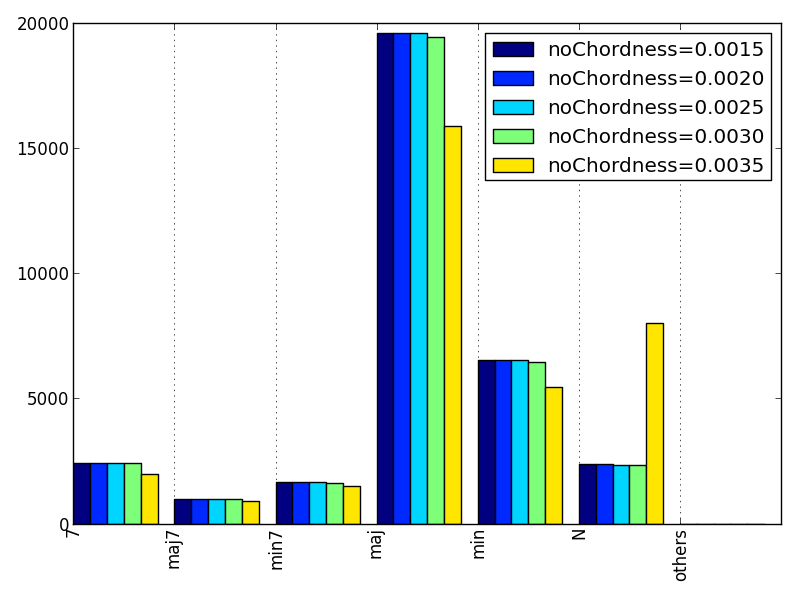
\includegraphics[scale=0.38]{errors/noChordness4a} \\ б)}
  \end{minipage}
  \caption{Диаграмма ошибок для разных значений $L_N$}
  \label{img:noChordness}
\end{figure}


\medskip

Параметры шаблонов для аккордов не оказывают практически никакого влияния на
результат при распознавании только мажорных и минорных трезвучий. Для случая
септаккордов они влияют только на количество ошибок, связанных с определением
септаккорда вместо трезвучия, но не на качество распознавания септаккордов само
по себе. Из реализованных эвристик имеет смысл применять только исправление
одиночных аккордов. Пороговое значение для определения отсутствия аккорда не
оказывает существенного влияния на результат.

% Для выбранного способа классификации векторов признаков необходимо определить
% наилучшие значения следующих параметров:
% \begin{enumerate}
%   \item расстояние (евклидово, косинусное, Кульбака-Ляйблера)
% \end{enumerate}

% Из перечисленных видов ошибок наиболее серьёзными являются тональные. Именно на
% их исправление нацелены все предлагаемые улучшения в алгоритмы распознавания
% аккордов. В некоторых случаях для их исправления может быть задействовано знание
% тональности. Это может помочь для исправления ошибок с определением минорного
% аккорда вместо соответствующего мажорного. Однако, например, аккорды C и G
% (\emph{до-мажор} и \emph{соль-мажор}) одинаково допустимы как для тональности
% \emph{до-мажор}, так и для тональности \emph{соль-мажор}), и различаются лишь
% своими функциями в рамках этих тональностей. Поэтому для исправления ошибки
% определения аккорда G вместо аккорда C необходима дополнительная информация,
% например, о ритмической структуре композиции. Также для исправления этих ошибок
% полезным может оказаться более точное и качественное вычисление спектрограммы,
% например, с использованием гребёнки очень точных фильтров. Здесь также играют
% роль и точное определение частоты настройки и ритма, и подавление шумов.
% 
% Исправление ошибок, связанных с отсутствием аккорда, имеет меньшую ценность. Как
% правило, для человека ясно, в каких местах композиции не звучат никакие аккорды.
% Также, вероятно, что определённые в этих фрагментах аккорды не будут
% соответствовать тональности композиции. Эти фрагменты можно пометить как
% подозрительные или исключить из индекса в случае автоматической индексации
% большого массива звукозаписей. Для случая ошибочного определения отсутствия
% аккорда ошибка также будет очевидной для человека и может быть исправлена
% повторным анализом с обязательным определением аккордов.
% 
% Проблема невозможных для метода аккордов не является существенной в том смысле,
% что действительно сложные и нестандартные аккорды встречаются достаточно редко.

% TODO ПРИМЕРЫ композиций, где эвристики работают и где не работают.

% Это вызвано как недостаточно аккуратным
%  определением отсутствия аккорда, так и тем, что все участки перед первой и
%  после последней определенной метрической доли считаются не содержащими
%  аккордов, что не всегда верно. 2 обратные ошибки (совокупной длительностью
%  252.99 с) вызваны, опять же, недостаточно аккуратным определением отсутствия
%  аккорда, а также отдельными сложными для анализа композициями. Так, в
%  композиции \emph{Queen -- We Will Rock You}, в соответствии с разметкой,
%  отсутствуют звучащие аккорды в течение первых 92 секунд (из 122 секунд общей
%  продолжительности). А композиция \emph{The Beatles -- Revolution 9} лишь в
%  некоторых фрагментах может рассматриваться как музыкальная звукозапись; её
%  разметка также содержит продолжительные участки, не содержащие звучащих
%  аккордов.

\section{Результаты MIREX Audio Chord Estimation 2013}

Реализованный в рамках данной работы алгоритм был выставлен на ежегодное
соревнование среди систем распознавания аккордов \emph{MIREX Audio Chord
Estimation 2013} \cite{ACEMirex20092013}, \cite{ACEBillboard20122013},
\cite{ACEBillboard20132013}. Диаграммы результатов представлены на рисунках
\ref{img:ACE2013_Mirex2009}, \ref{img:ACE2013_Billboard2012} и
\ref{img:ACE2013_Billboard2013}.

\begin{figure} [htbp] 
  \center
  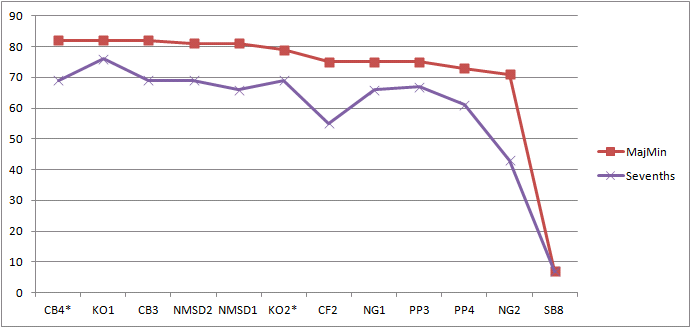
\includegraphics [scale=0.55] {ACE2013_Mirex2009}
  \caption{Результаты MIREX ACE 2013 на коллекции Mirex2009}
  \label{img:ACE2013_Mirex2009}  
\end{figure}

\begin{figure} [htbp] 
  \center
  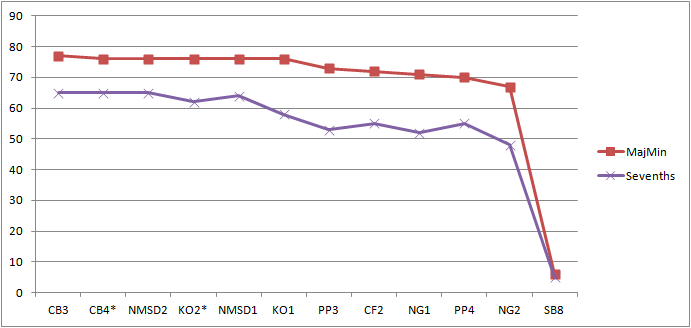
\includegraphics [scale=0.55] {ACE2013_Billboard2012}
  \caption{Результаты MIREX ACE 2013 на коллекции Billboard2012}
  \label{img:ACE2013_Billboard2012}  
\end{figure}

\begin{figure} [htbp] 
  \center
  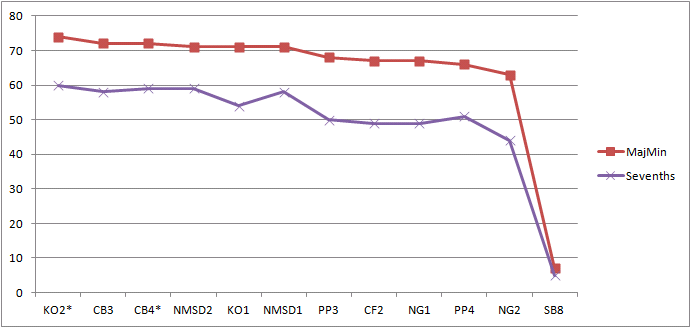
\includegraphics [scale=0.55] {ACE2013_Billboard2013}
  \caption{Результаты MIREX ACE 2013 на коллекции Billboard2013}
  \label{img:ACE2013_Billboard2013}  
\end{figure}

Как видно, описанный в главе \ref{chapt1} метод показывает сравнимые с другими
участниками результаты. При этом все остальные алгоритмы используют методы
машинного обучения. Версия алгоритма под названием NG2 отличается от NG1 только
тем, что содержит шаблоны для мажорного и минорного септаккордов, а также для
доминантсептаккорда. За счёт ошибочного определения септаккордов вместо обычных
мажорного или минорного аккорда версия NG2 показала более слабый результат.

Можно заметить, что все алгоритмы показывают более слабый результат на
коллекциях \emph{Billboard 2012} и \emph{Billboard2013}, недоступных для
участников, чем на широко используемой много лет подряд коллекции
\emph{Isophonics}. В случае, когда от алгоритмов требуется распознавать
септаккорды, результаты также падают. Интересно, что даже наилучшие из
алгоритмов незначительно превышают значение $0.8$ для взвешенного среднего
перекрытия, и до сих пор никому не удалось добиться существенного прогресса в
качестве распознавания. Исключением являются случаи переобучения (пример
приведен в \cite{BoulangerLewandowski2013}, когда алгоритм обучается и
тестируется на одной и той же коллекции. Очевидно, что в данном случае
сравнение с результатами, полученными при обучении и тестировании на разных
коллекциях, некорректны.

\section{Быстродействие} \label{sect3_time}

Метод должен обладать достаточным быстродействием для того, чтобы его
использование для решения реальных задач было целесообразным. В данном разделе
анализируется производительность реализованного метода в зависимости от значений
параметров.

Весь процесс обработки звукового файла можно разделить на 4 стадии:
\begin{enumerate}
  \item определение частоты настройки музыкальных инструментов;
  \item определение ритма при помощи внешней библиотеки;
  \item вычисление спектрограммы;
  \item преобразования спектрограммы и распознавание аккордов.
\end{enumerate}

Процесс распознавания аккордов при наличии последовательности хроматических
векторов отнимает очень небольшое время, и поэтому не был выделен в отдельную
стадию. Однако вычисление преобразований спектрограммы уже отнимает заметное
время. При использовании нейронной сети все дополнительные затраты времени на её
обучение также могут быть отнесены к этой стадии.

На быстродействие алгоритма определения ритма автор повлиять не может.
Длительность остальных стадий обработки файла зависит от параметров метода.
Наибольшее влияние оказывают количество компонент преобразования постоянного
качества (количество октав и количество компонент на октаву $N_0$) и
коэффициент $T$, соответствующий количеству вычислений спектра звука,
приходящихся на одну метрическую долю. Именно эти параметры задают количество
преобразований постоянного качества, которые необходимо вычислить для получения
спектрограммы звукозаписи, и количество участвующих в каждом преобразовании
значений.

Полностью процесс распознавания аккордов в используемой коллекции из 318
композиций общей длительностью около 17 ч 8 мин отнимает примерно 4 ч 15 мин при
следующих условиях:
\begin{itemize}
  \item компьютер с процессором Intel Core i5 с тактовой частотой 2.8 ГГц;
  \item вычисления в 3 потока;
  \item $N_0=36$, охват 6 октав, начиная со звука \emph{до} большой октавы
  (65.4 Гц);
  \item $T=8$.
\end{itemize}
Взвешенное среднее перекрытие и сегментация для каждой композиции из
используемой коллекции представлены в приложении \ref{AppendixA}.

При тех же условиях (но с использованием 4 потоков) только наиболее
продолжительные действия -- определение частоты настройки и получение
спектрограммы (при известных моментах начала метрических долей и без
дополнительных преобразований) -- занимают примерно 3 ч 40 мин. В таблице
\ref{TTimeN0} показано время выполнения этих же действий при разных значениях
$N_0$. При использовании $N_0=60$, несмотря на большее время работы, прирост
качества распознавания аккордов практически не заметен (см. таблицу \ref{TN0}).
При $N_0=12$ выигрыш во времени невелик, при этом ухудшение результата очень
заметно.

\begin{table} [htbp]
  \centering
  \parbox{15cm}{\caption{Совокупная продолжительность определения частоты
  настройки и вычисления спектрограммы}
  \label{TTimeN0}}
  \begin{tabular}{|l|l|}
  \hline
  $N_0$ & Время \\
  \hline
  12 & 2 ч 59 мин 2 с \\
  36 & 3 ч 37 мин 47 с \\
  60 & 4 ч 23 мин 27 с\\
  \hline
  \end{tabular}
\end{table}

Зависимость времени вычисления от коэффициента $T$ была исследована при
$N_0=36$, охват 4 октавы, начиная со звука \emph{до} большой октавы (65.4 Гц).
Результаты показаны в таблице \ref{TTimeT}. В отличие от $N_0$, параметр $T$ не
так существенно влияет на качество распознавания аккордов (см. таблицу
\ref{TTw}). Поэтому алгоритм можно использовать при $T=2$, когда быстродействие
алгоритма важнее, чем небольшой выигрыш в качестве распознавания.

\begin{table} [htbp]
  \centering
  \parbox{15cm}{\caption{Совокупная продолжительность определения аккордов при
  разных значениях параметра $T$}
  \label{TTimeT}}
  \begin{tabular}{|l|l|}
  \hline
  $T$ & Время \\
  \hline
  2 & 1 ч 31 мин 4 с \\
  4 & 1 ч 58 мин 51 с \\
  8 & 3 ч 1 мин 58 с \\
  \hline
  \end{tabular}
\end{table}

Время, затрачиваемое на обучение нейронной сети, оказывается на практике
достаточно заметным. Однако, как видно из таблицы \ref{TTimeConf}, добавление
каждого нового слоя существенно увеличивает время обучения при незначительном
улучшении результата (см. таблицу \ref{Tnnconf}). Добавление рекуррентных
соединений резко увеличивает время обучения по сравнению с аналогичной
нерекуррентной сетью. Кроме того, из-за наличия зависимости от значений
предыдущего шага не удаётся эффективно вычислять выходные значения во время
тестов, из-за чего продолжительность тестов также резко возрастает.

\begin{table} [htbp]
  \centering
  \parbox{15cm}{\caption{Совокупная продолжительность обучения и тестов при
  разных конфигурациях нейронной сети}
  \label{TTimeConf}}
  \begin{tabular}{|l|l|l|}
  \hline
  Конфигурация & Продолжительность обучения & Продолжительность тестов \\
  \hline
  SDA (60, 100) & 43 мин 49 с & 4 мин 38 с \\
  SDA (60, 200) & 1 ч 2 мин 19 с & 4 мин 56 с \\
  SDA (60, 300) & 1 ч 20 мин 48 с & 5 мин 17 с \\
  SDA (60, 200, 100) & 2 ч 19 мин 52 с & 7 мин 6 с \\
  SDA (60, 300, 300) & 6 ч 21 мин 28 с & 8 мин 18 с \\
  SDA (60, 300, 300, 300) & 15 ч 21 мин 19 с & 13 мин 21 с \\
  RSDA (60, 300) & 6 ч 55 мин 43 с & 1 ч 52 мин 01 с\\
  \hline
  \end{tabular}
\end{table}

\section{Выводы}

\begin{enumerate}
  \item Произведён анализ влияния параметров реализованного метода на качество
  распознавания аккордов и скорость работы метода. Определена степень влияния
  каждого из параметров на качество распознавания аккордов.
  \item Определены параметры, наиболее сильно влияющие на быстродействие метода;
  показано, что можно добиться прироста скорости при незначительном снижении
  качества распознавания.
  \item Реализованный алгоритм показал хороший результат в международном
  соревновании среди алгоритмов распознавания аккордов \emph{MIREX Audio Chord
  Estimation 2013}.
\end{enumerate}

%\newpage
%============================================================================================================================

\clearpage